\documentclass[reqno,12pt,letterpaper]{amsart}
\RequirePackage{amsmath,amssymb,amsthm,graphicx,mathrsfs,url,slashed}
\RequirePackage[usenames,dvipsnames]{xcolor}
\RequirePackage[colorlinks=true,linkcolor=Red,citecolor=Green]{hyperref}
\RequirePackage{amsxtra}
\usepackage{cancel}
\usepackage{tikz-cd}

\setlength{\textheight}{9.3in} \setlength{\oddsidemargin}{-0.25in}
\setlength{\evensidemargin}{-0.25in} \setlength{\textwidth}{7in}
\setlength{\topmargin}{-0.25in} \setlength{\headheight}{0.18in}
\setlength{\marginparwidth}{1.0in}
\setlength{\abovedisplayskip}{0.2in}
\setlength{\belowdisplayskip}{0.2in}
\setlength{\parskip}{0.05in}
\renewcommand{\baselinestretch}{1.05}

\title[Riemannian least-gradient maximum principle]{The least-gradient maximum principle on Riemannian manifolds}
\author{Aidan Backus}
\date{May 2022}

\newcommand{\NN}{\mathbf{N}}
\newcommand{\ZZ}{\mathbf{Z}}
\newcommand{\QQ}{\mathbf{Q}}
\newcommand{\RR}{\mathbf{R}}
\newcommand{\CC}{\mathbf{C}}
\newcommand{\DD}{\mathbf{D}}
\newcommand{\PP}{\mathbf P}
\newcommand{\MM}{\mathbf M}
\newcommand{\II}{\mathbf I}
\newcommand{\Hyp}{\mathbf H}
\newcommand{\Sph}{\mathbf S}
\newcommand{\Group}{\mathbf G}
\newcommand{\GL}{\mathbf{GL}}
\newcommand{\Orth}{\mathbf{O}}
\newcommand{\SpOrth}{\mathbf{SO}}
\newcommand{\Ball}{\mathbf{B}}

\DeclareMathOperator*{\Expect}{\mathbf E}

\DeclareMathOperator{\avg}{avg}
\DeclareMathOperator{\card}{card}
\DeclareMathOperator{\cent}{center}
\DeclareMathOperator{\ch}{ch}
\DeclareMathOperator{\codim}{codim}
\DeclareMathOperator{\diag}{diag}
\DeclareMathOperator{\diam}{diam}
\DeclareMathOperator{\dom}{dom}
\DeclareMathOperator{\Exc}{Exc}
\DeclareMathOperator{\Gal}{Gal}
\DeclareMathOperator{\Hom}{Hom}
\DeclareMathOperator{\Iso}{Iso}
\DeclareMathOperator{\Jac}{Jac}
\DeclareMathOperator{\Lip}{Lip}
\DeclareMathOperator{\Met}{Met}
\DeclareMathOperator{\id}{id}
\DeclareMathOperator{\rad}{rad}
\DeclareMathOperator{\rank}{rank}
\DeclareMathOperator{\Rm}{Rm}
\DeclareMathOperator{\Hess}{Hess}
\DeclareMathOperator{\Hol}{Hol}
\DeclareMathOperator{\Radon}{Radon}
\DeclareMathOperator*{\Res}{Res}
\DeclareMathOperator{\sgn}{sgn}
\DeclareMathOperator{\singsupp}{sing~supp}
\DeclareMathOperator{\Spec}{Spec}
\DeclareMathOperator{\supp}{supp}
\DeclareMathOperator{\Tan}{Tan}
\newcommand{\tr}{\operatorname{tr}}

\newcommand{\Ric}{\mathrm{Ric}}
\newcommand{\Riem}{\mathrm{Riem}}
\newcommand*\dif{\mathop{}\!\mathrm{d}}
\newcommand*\Dif{\mathop{}\!\mathrm{D}}
\newcommand{\LapQL}{\Delta^{\mathrm{ql}}}

\newcommand{\dbar}{\overline \partial}

\DeclareMathOperator{\atanh}{atanh}
\DeclareMathOperator{\csch}{csch}
\DeclareMathOperator{\sech}{sech}

\DeclareMathOperator{\Div}{div}
\DeclareMathOperator{\Gram}{Gram}
\DeclareMathOperator{\grad}{grad}
\DeclareMathOperator{\dist}{dist}
\DeclareMathOperator{\spn}{span}
\DeclareMathOperator{\Ell}{Ell}
\DeclareMathOperator{\WF}{WF}

\newcommand{\Lagrange}{\mathscr L}
\newcommand{\DirQL}{\mathscr D^{\mathrm{ql}}}
\newcommand{\DirL}{\mathscr D}

\newcommand{\Hilb}{\mathcal H}
\newcommand{\Homology}{\mathrm H}
\newcommand{\normal}{\mathbf n}
\newcommand{\radial}{\mathbf r}
\newcommand{\evect}{\mathbf e}
\newcommand{\vol}{\mathrm{vol}}

\newcommand{\pic}{\vspace{30mm}}
\newcommand{\dfn}[1]{\emph{#1}\index{#1}}

\renewcommand{\Re}{\operatorname{Re}}
\renewcommand{\Im}{\operatorname{Im}}

\newcommand{\loc}{\mathrm{loc}}
\newcommand{\cpt}{\mathrm{cpt}}

\def\Japan#1{\left \langle #1 \right \rangle}

\newtheorem{theorem}{Theorem}[section]
\newtheorem{badtheorem}[theorem]{``Theorem"}
\newtheorem{prop}[theorem]{Proposition}
\newtheorem{lemma}[theorem]{Lemma}
\newtheorem{sublemma}[theorem]{Sublemma}
\newtheorem{claim}[theorem]{Claim}
\newtheorem{proposition}[theorem]{Proposition}
\newtheorem{corollary}[theorem]{Corollary}
\newtheorem{conjecture}[theorem]{Conjecture}
\newtheorem{axiom}[theorem]{Axiom}
\newtheorem{assumption}[theorem]{Assumption}

\theoremstyle{definition}
\newtheorem{definition}[theorem]{Definition}
\newtheorem{remark}[theorem]{Remark}
\newtheorem{example}[theorem]{Example}
\newtheorem{notation}[theorem]{Notation}

\newtheorem{exercise}[theorem]{Discussion topic}
\newtheorem{homework}[theorem]{Homework}
\newtheorem{problem}[theorem]{Problem}

\makeatletter
\newcommand{\proofpart}[2]{%
  \par
  \addvspace{\medskipamount}%
  \noindent\emph{Part #1: #2.}
}
\makeatother

\newtheorem{ack}{Acknowledgements}

\numberwithin{equation}{section}


% Mean
\def\Xint#1{\mathchoice
{\XXint\displaystyle\textstyle{#1}}%
{\XXint\textstyle\scriptstyle{#1}}%
{\XXint\scriptstyle\scriptscriptstyle{#1}}%
{\XXint\scriptscriptstyle\scriptscriptstyle{#1}}%
\!\int}
\def\XXint#1#2#3{{\setbox0=\hbox{$#1{#2#3}{\int}$ }
\vcenter{\hbox{$#2#3$ }}\kern-.6\wd0}}
\def\ddashint{\Xint=}
\def\dashint{\Xint-}

\usepackage[backend=bibtex,style=alphabetic]{biblatex}
\renewcommand*{\bibfont}{\normalfont\footnotesize}
\addbibresource{topics.bib}
\renewbibmacro{in:}{}
\DeclareFieldFormat{pages}{#1}


\begin{document}
\begin{abstract}
The least-gradient maximum principle, essentially due to Miranda and de Giorgi in the 1960s, shows that least-gradient functions define a minimal lamination of the support of their derivative.
We show that this result still holds on hyperbolic manifolds.
As a consequence we answer some questions of Daskalopoulos--Uhlenbeck concerning the $L^\infty$-Teichm\"uller theory.
\end{abstract}

\maketitle

%%%%%%%%%%%%%%%%%%%%%%%%%%%%%%%%%%%%%%%%%%%%%%%%%%%%%%%

% \tableofcontents

\section{Introduction}
Throughout this paper, let $M$ be an oriented Riemannian manifold of metric $g$ and dimension $d$.
For a function $u \in BV_\loc(M)$, we write $\star |\dif u|$ for the total variation of the derivative, c.f. (\ref{total variation}).

\begin{definition}\label{main definitions}
A function $u \in BV_\loc(M)$ has \dfn{least gradient} if for every $v \in BV_\cpt(M)$ such that $\supp v \subseteq U \Subset M$,
$$\int_U \star |\dif u| \leq \int_U \star |\dif u + \dif v|.$$
A set $U$ of locally finite perimeter has \dfn{least perimeter} if $1_U$ has least gradient.
\end{definition}

Functions of least gradient arise naturally as solutions to an inverse problem in magnetic resonance imaging (MRI) \cite{Nachman2009, Tamasan2019, Joy09} as well as the formal limit of $p$-harmonic functions as $p \to 1$, but we are interested in them primarily because of their application to the $L^\infty$-Teichm\"uller theory of Thurston and Daskalopoulos--Uhlenbeck \cite{thurston1998minimal, daskalopoulos2020transverse}.
In that context one is interested in the existence and regularity of minimal laminations in a closed hyperbolic manifold, and our main theorem, Theorem \ref{main thm}, constructs them from function of least gradient.

\begin{definition}
A \dfn{minimal lamination} in $M$ is a partition of a closed subset of $M$ into smooth hypersurfaces with zero mean curvature.
\end{definition}

\begin{theorem}[maximum principle]\label{main thm}
Suppose that $2 \leq d \leq 7$ and let $M$ be locally homogeneous.
Let $u: M \to \RR$ be a function of least gradient, and $A_y = \partial \{u > y\}$.
Then $\lambda = (A_y)_{y \in \RR}$ is a minimal lamination in $M$, and each $A_y$ is a locally finite union of connected minimal hypersurfaces.
\end{theorem}

Theorem \ref{main thm} generalizes \cite[Proposition 3.4]{górny2017planar} and partially solves a problem \cite[Problem 9.5]{daskalopoulos2020transverse} of Daskalopoulos--Uhlenbeck; we state this as Corollary \ref{maximum stretch contains lamination}.
As a byproduct we obtain Corollary \ref{ruelle sullivan antiderivative} which is a solution to \cite[Problem 9.7]{daskalopoulos2020transverse}.
Moreovevr, it was shown by G\'orny \cite[Theorem 1.2]{górny2017planar} that functions of least gradient on $\RR^d$, $d \leq 7$, have a decomposition into continuous and jump parts.
Given Theorem \ref{main thm}, the proof of this result goes through verbatim: TODO CHECK ME

\begin{theorem}[G\'orny's regularity theorem]\label{Gorny regularity}
Let $M$ be an open bounded strictly convex manifold of dimension $\leq 7$.
Then any function of least gradient $u: M \to \RR$ can be written as the sum of a continuous function of least gradient, and a function of least gradient with only jump discontinuities.
\end{theorem}

%%%%%%%%%%%%%%%%%%%%%%%%%%%%%%%%%%%%%
\subsection{Overview of the proof}
Regularity proofs in geometric measure theory usually have three components:
\begin{enumerate}
\item A monotonicity formula that controls the behavior of a singular set at fine scales;
\item Study of the tangent cone obtained by blowing up a singular set;
\item A $\varepsilon$-regularity lemma which asserts that a singular set of ``small oscillation'' is smooth.
\end{enumerate}
Experts in PDE can understand the study of the tangent cone as a proof of ``subcriticality'', as these tangent cones should be thought of as ``zero solutions''; then the $\varepsilon$-regularity lemma is a sort of ``small data well-posedness''.
For an exposition of this strategy in the case of minimal currents in euclidean space see Federer \cite[\S5.3]{federer2014geometric}.
More relevant to our work, we note that this strategy was also used by Miranda to show the least-gradient maximum principle on euclidean space \cite{Miranda64, Miranda66, Miranda67}.
We shall follow Giusti's exposition \cite{Giusti77} of Miranda's proof, and shall often refer to Giusti when the proof of a lemma is straightforward to generalize from the euclidean case.

Before the proof, we give some applications of Theorem \ref{main thm} and some open problems in this present section.
In \S\ref{LeastGradientFunctions} we recall elementary facts about functions of least gradient and their level sets, the so-called sets of least perimeter, c.f. Proposition \ref{level sets are minimal}.
We then show that the tangent cone of a set of least perimeter exists and is actually a hyperplane, Proposition \ref{blowup theorem}; this can easily be shown by reduction to the Bernstein-Fleming theorem which classifies minimal cones in $\RR^d$ \cite[Theorem 17.3]{Giusti77}.

In \S\ref{MollifierSection} we prove the following monotonicity formula which may be of independent interest:

\begin{theorem}[monotonicity formula]\label{monotonicity prestate}
There exists $A \geq 0$ depending continuously on $P \in M$ such that for every function $u$ of least gradient defined near $P \in M$, every normal coordinate system $(x^\mu)$ based at $P$, and $0 < r_1 < r_2 \lesssim 1$,
\begin{align*}
&\left|\int_{r_1}^{r_2} \partial_r \left[r^{1 - d} \int_{B(P, r)} \dif u \wedge \dif x^1 \wedge \cdots \wedge \dif x^{d - 1}\right] \dif r\right|^2 \\
&\qquad \lesssim \left(1 + (d - 1) \log \frac{r_2}{r_1}\right) \left(r_2^{1 - d}\int_{B(P, r_2)} \star |\dif u| \right)\left(\int_{r_1}^{r_2} \partial_r \left[e^{Ar^2} r^{1 - d} \int_{B(P, r)} \star |\dif u|\right] \dif r\right).
\end{align*}
\end{theorem}

This formula generalizes \cite[Theorem 2.8]{Miranda66} and is stronger than monotonicity formulae for minimal surfaces in Riemannian manifolds that the author is aware of (see e.g. the notes of Marques \cite[\S7]{MarquesXX}) in that it gives a lower bound on the rate of growth of the monotone quantity $e^{Ar^2} r^{1 - d} \int_{B_r} \star |\dif u|$.
As a consequence, we show Proposition \ref{mollifier quant}, which allows for the mollification of sets of least perimeter.

We thus restrict to $C^1$ sets of least perimeter in \S\ref{Plateau section}, and represent them as graphs of solutions $\omega: \Omega \to \RR$ of a Plateau equation (Proposition \ref{construction of Plateau energy}) where $\Omega$ is a certain Riemannian manifold constructed from $M$.
In particular, if $M$ is homogeneous, then we can assume that the metric on $M$ is written in ``Killing gauge", a gauge condition which implies that $\Omega$ does not depend on the given $C^1$ set.
This drastically reduces the complexity of the Plateau equation.

We then arrive at the fundamental inequality of this paper: Proposition \ref{dGL Laplace} generalizes \cite[Teorema 4.3]{Miranda66} and shows that one obtains a multiplicative gain in the oscillation of $\omega$ when one passes from a scale $r$ to $r/2$, as long as $g$ is in Killing gauge.

In \S\ref{de Giorgi section} our goal is to show:

\begin{theorem}[regularity of minimal hypersurfaces]\label{main lma}
Suppose that $2 \leq d \leq 7$.
Then every set of least perimeter in $M$ is bounded by a minimal hypersurface.
\end{theorem}

Theorem \ref{main lma} follows from the de Giorgi $\varepsilon$-regularity lemma, Proposition \ref{dGL final}, which generalizes \cite[Teorema 5.7]{Miranda66} and itself follows by a mollification of Proposition \ref{dGL Laplace}.

Let us now explain why Theorem \ref{main thm} follows from Theorem \ref{main lma}.
Let $u$ have least gradient,
\begin{equation}\label{lamination union}
A = \bigcup_y \partial \{u > y\},
\end{equation}
let $B$ be the interior of $\{du = 0\}$, and let $x \in M$.
Then $x \in B$ iff $u = u(x)$ near $x$, but that happens iff for every $y < u(x)$, $x$ is interior to $\{u > y\}$ and for every $y \geq u(x)$, $x$ is exterior to $\{u > y\}$.
This happens iff for every $y \in \RR$, $x$ is either interior or exterior to $\{u > y\}$, thus $x \notin \partial \{u > y\}$, which happens iff $x \notin A$.
Thus $\{A, B\}$ is a partition of $M$, so $A$ is closed.
Moreover, the sets $\{u > y\}$ are totally ordered by $\subseteq$, so the sets $\partial \{u > y\}$ are disjoint.
They are also hypersurfaces with the desired amount of regularity, by Theorem \ref{main lma}.
By Proposition \ref{local finiteness} the decomposition of $\partial \{u > y\}$ into connected components is locally finite.

%%%%%%%%%%%%%%%%%%%%%%%%%%%%%%%%%%%%%%%%%%%%%%%

\subsection{Applications to hyperbolic geometry}
The Thurston asymmetric metric, first defined in \cite{thurston1998minimal}, is constructed from best-Lipschitz maps between two closed hyperbolic manifolds.
As a first step towards an analytic understanding of the Thurston asymmetric metric, Daskalopoulos--Uhlenbeck \cite{daskalopoulos2020transverse} considered best-Lipschitz maps $M \to \Sph^1$ where $M$ is a closed hyperbolic surface.
They identified a particularly important class of such maps, the $\infty$-harmonic maps, defined as follows, which are particularly significant because they induce geodesic laminations of $M$.

\begin{definition}
If a function $u$ is the weak limit in $L^r$ for $r > d$ of $p$-harmonic functions as $p \to \infty$, we call $u$ \dfn{$\infty$-harmonic}.
For an $\infty$-harmonic function $u$ we define the \dfn{maximum-stretch locus}
$$\lambda_u := \{x \in M: L(x) = \sup L\}$$
where $L(x)$ denotes the local Lipschitz constant of $u$ at $x$.
\end{definition}

\begin{theorem}\label{infinity harmonic laminations}
Suppose that $M$ is a closed hyperbolic surface and $u$ is an $\infty$-harmonic function. Then the maximum-stretch locus $\lambda_u$ is a geodesic lamination in $M$.
\end{theorem}

In \cite[\S5]{daskalopoulos2020transverse}, Daskalopoulos--Uhlenbeck prove Theorem \ref{infinity harmonic laminations} by considering the viscosity solution theory of $\infty$-Laplace equation
\begin{equation}\label{infinity laplace}
    \Hess u(\grad u, \grad u) = 0.
\end{equation}
However, the theory of viscosity solutions of (\ref{infinity laplace}) is still nascent, and Daskalopoulos--Uhlenbeck ask for a proof of Theorem \ref{infinity harmonic laminations} that bypasses (\ref{infinity laplace}) altogether, c.f. \cite[Problem 9.5]{daskalopoulos2020transverse}.
We give a partial resolution of this problem by proving \cite[Theorem-Conjecture 9.6]{daskalopoulos2020transverse}.
Before stating it we note that by a \dfn{section of least gradient} on $M$ we mean a section that lifts to a function of least gradient on $\Hyp^d$.

\begin{corollary}\label{maximum stretch contains lamination}
Let $u$ be an $\infty$-harmonic function on a closed hyperbolic surface $M$.
Then the maximum-stretch locus $\lambda_u$ contains a geodesic lamination.
\end{corollary}
\begin{proof}
By \cite[\S6]{daskalopoulos2020transverse}\footnote{The proof that such a section exists does not use Theorem \ref{infinity harmonic laminations}.}, there exists an affine bundle $E \to M$ and a section $v$ of least gradient of $E$ such that $\supp \dif v \subseteq \lambda_u$.
By Theorem \ref{main thm}, $\supp \dif v$ is a geodesic lamination.
\end{proof}

It is not clear that $\supp \dif v = \lambda_u$ in the above corollary, but see Conjecture \ref{two laminations agree}.

Daskalopoulos--Uhlenbeck also ask for \cite[Problem 9.7]{daskalopoulos2020transverse} a partial converse to the fact that $\dif v$ endows $\lambda_u$ with the structure of an oriented measured lamination, which we now prove.
For the definitions, see \cite[\S8]{daskalopoulos2020transverse} or the original paper of Ruelle--Sullivan \cite{Ruelle75}.

\begin{corollary}\label{ruelle sullivan antiderivative}
Let $\lambda$ be an oriented, transversely measured geodesic lamination on a closed hyperbolic surface $M$, and let $\dif v$ be the Ruelle-Sullivan $1$-current induced by $\lambda$.
Then $\dif v$ is the derivative of a section of least gradient $v: M \to E$, for some affine bundle $E \to M$.
\end{corollary}
\begin{proof}
As observed in \cite[\S9]{daskalopoulos2020transverse}, if we lift $\dif v$ to a $1$-current $\dif \tilde v$ on $\Hyp^2$, then $\dif \tilde v$ is exact and any antiderivative $\tilde v$ of $\dif \tilde v$ has superlevel sets $\{\tilde v \geq y\}$ which are bounded by geodesics.
Moreover we can choose $\tilde v$ to be $\pi_1(M)$-equivariant.
The claim now follows from Proposition \ref{minimal bounding implies least gradient} and the realization of $\pi_1(M)$-equivariant functions on $\Hyp^2$ as sections of an affine bundle \cite[\S4]{daskalopoulos2020transverse}.
\end{proof}

The analogous theory for threefolds is also quite interesting, as closed minimal surfaces in hyperbolic threefolds have been studied intensely since the seminal work of Uhlenbeck \cite{Uhlenbeck1983ClosedMS}.
Daskalopoulos--Uhlenbeck have suggested \cite[Problem 9.13]{daskalopoulos2020transverse} that for a line bundle $E \to M$ over a closed hyperbolic threefold $M$, it would be particularly fruitful to study sections of $E$ of least gradient.
However, we shall not pursue this line of inquiry here.

Theorem \ref{main thm} also furnishes a large class of minimal laminations which are inexpensive to numerically compute.

\begin{proposition}\label{cohomology makes laminations}
Let $M$ be a closed hyperbolic manifold of dimension $d \leq 7$, and let $\alpha \in H^1(M, \RR)$.
Then there is a natural minimal lamination $\lambda$ in $M$ induced by $\alpha$, which can be obtained by solving a least-gradient Dirichlet problem on a fundamental polytope of $M$.
\end{proposition}
\begin{proof}
Let $\Gamma = \pi_1(M)$. The Hurcewiz theorem implies that $\alpha$ pulls back to a map $\Gamma \to \RR$.
Then $\alpha$ is a representation of $\Gamma$ and thus induces a space $E$ of equivariant functions on the boundary $\Omega$ of each fundamental polytope $\Omega$ of $\Gamma$. To be more precise, for every $f \in E$ and $\gamma \in \Gamma$,
\begin{equation}\label{boundary data for Loisel}
f(\gamma x) = f(x) + \alpha(\gamma),
\end{equation}
and $f$ is constant on each face of $\partial \Omega$.
The relation (\ref{boundary data for Loisel}) is an underdetermined boundary condition for functions in $E$, and so we consider the subspace $E'$ of functions which in addition are zero on a maximal set of faces such that we do not determine $f|\partial \Omega = 0$, thus any function $E' \subseteq E$ has a completely determined trace $t$ on $\partial \Omega$.
It follows from \cite[Theorem 4.4]{daskalopoulos2020transverse} that there exists a function $u$ of least gradient on $\Omega$ whose trace is $t$.
The minimal lamination induced by a function $u \in E$ of least gradient from Theorem \ref{main thm} does not depend on the class of $u$ in $E/E'$, since that is a space of constants; so we obtain a uniquely defined minimal lamination of $M$.
\end{proof}

\begin{corollary}
With $M, \alpha, \lambda$ as in Proposition \ref{cohomology makes laminations}, and every quasiuniform triangulation $T$ of $M$, there exists a numerical algorithm for computing $\lambda$ with finite elements in $T$ with time complexity $O(|T|^{1/2} \log |T|)$ where $|\cdot|$ is cardinality.
\end{corollary}
\begin{proof}
By \cite[Theorem 1]{Loisel20}, one can solve the least-gradient Dirichlet problem with finite elements in $T$ with time complexity $O(|T|^{1/2} \log |T|)$.
\end{proof}

TODO: Do some numerical experiments, show what minimal laminations in a fundamental polytope in $\Hyp^3$ look like


%%%%%%%%%%%%%%%%%%%%%%%%%%%%%%%%%%%%%%%%%%%%%%%

\subsection{Some open problems}
We believe that Theorem \ref{main lma} could be extended to a wider class of Riemannian manifolds:

\begin{conjecture}\label{main conj}
Theorem \ref{main lma} holds without any homogeneity assumption.
\end{conjecture}

It seems highly unlikely that Theorem \ref{main lma} can be extended to any manifold $M$ of dimension $8$, due to the existence of Simons cones in $\RR^8$ \cite[Theorem A]{BOMBIERI1969}.
We would therefore appreciate a general class of counterexampels:

\begin{problem}
For each Riemannian manifold $M$ of dimension $8$, construct a set $U$ of least perimeter in $M$ such that $\partial U$ has a singularity of codimension $8$.
\end{problem}

Owing to the G\'orny regularity theorem, Theorem \ref{Gorny regularity}, we suspect that its consequence \cite[Theorem 1.1]{górny2017planar} holds, giving well-posedness for the Dirichlet problem in strictly convex planar domains.
However, this is not obvious as we have not extended the Sternberg--Williams--Ziemer theorem \cite{ZiemerWilliamsSternberg1992} to the Riemannian case.
Since the only homogeneous spaces of dimension $2$ have constant curvature, it is natural to restrict to the cases of $\Hyp^2$ or $\Sph^2$ in the below conjecture.

\begin{conjecture}
Let $\overline M = M \cup \partial M$ be a compact, strictly convex submanifold-with-boundary of $\Hyp^2$, or a closed, strictly convex submanifold-with boundary of $\Sph^2$ such that $\Sph^2 \setminus \overline M$ is nonempty.
Then there exists a solution of the least-gradient Dirichlet problem on $M$ with data in $BV(\partial M)$.
\end{conjecture}

We would also like to know that the $\infty$-harmonic/least-gradient duality gives a complete proof of Theorem \ref{infinity harmonic laminations}, which follows from the below conjecture.

\begin{conjecture}\label{two laminations agree}
Let $u$ be an $\infty$-harmonic function with dual least-gradient section $v$.
Then $\supp \dif v = \lambda_u$.
\end{conjecture}


%%%%%%%%%%%%%%%%%%%%%%%%%%%%%%%%%%%%%%%%%%%%%%%%

\subsection{Acknowledgements}
I would like to thank Georgios Daskalopoulos for suggesting this project and for many helpful discussions.
I would also like to thank Trent Lucas for comments on Proposition \ref{cohomology makes laminations} and Joshua Lin for providing me with Proposition \ref{Josh helped}.



%%%%%%%%%%%%%%%%%%%%%%%%%%%%%%%%%%%%%%%%%%%%%%%%%%

\section{Functions of least gradient}\label{LeastGradientFunctions}
\subsection{Riemannian measure theory}
We begin by fixing notation.
The statements $A \lesssim B$ and $A = O(B)$ are equivalent and mean that there exists $C > 0$ independent of $A, B \geq 0$ such that $A \leq BC$.
Similarly the statements $A \ll B$ and $A = o(B)$ mean that there exists a function $f: \RR_+ \to \RR_+$ with $\lim_{x \to 0} f(x) = 0$, such that $A \leq Bf(B)$.

The operator $\star$ is the Hodge star, thus $\star 1$ is the Riemannian volume form.
For tensor fields we shall use the musical isomorphisms $\sharp, \flat$ and the Einstein convention.
When using the Einstein convention, Greek indices range over $0, 1, \dots$ while Latin indices range over $1, \dots$.

We now recall the Riemannian analogue of the main results of \cite[Chapter 1]{Giusti77}.
We write $\int_U \omega \wedge \psi$ for the pairing of a de Rham $\ell$-current $\omega$ with a compactly supported $\ell$-form $\psi$ in an open set $U$. See \cite{simon1983GMT} for the definition of a de Rham current.
In particular, we have a Poincar\'e duality map which identifies a $d - \ell$-form $\omega$ with the $\ell$-current $\psi \mapsto \int_U \omega \wedge \psi$.

We identify the distributional derivative of a function $u$ with the $d-1$-current
$$\int_U \dif u \wedge \psi = -\int_U u \dif \psi.$$
A function $u$ is in $BV(U)$ iff its derivative $\dif u$ has finite total variation
\begin{equation}\label{total variation}
\int_U \star |\dif u| := \sup_{\substack{||\psi||_{L^\infty} \leq 1\\\supp \psi \Subset V}} \int_U \dif u \wedge \psi.
\end{equation}
Whether a current has locally finite total variation is independent of the Riemannian metric and so $BV_\loc(M)$ is also independently defined.

Now let $u \in BV_\loc(M)$.
Then by \cite[Theorem 4.14]{simon1983GMT}, there exists a $\star |\dif u|$-measurable section $f$ of the cosphere bundle $S'M$ such that for every compactly supported $d-1$-form $\psi$,
\begin{equation}\label{RNy formula}
\int_M \dif u \wedge \psi = \int_M f|\dif u| \wedge \psi.
\end{equation}

For a vector field $X$, we write $\star (Xu) := \dif u \wedge \star (X^\flat)$.
The section $f$ of (\ref{RNy formula}) is given pointwise $\star |\dif u|$-almost everywhere, in any local coordinates $(y^\mu)$, by
\begin{equation}\label{Lebesgue point definition}
    f(x) = \left[\lim_{r \to 0} \frac{\int_{B(x, r)} \star \partial_\mu u}{\int_{B(x, r)} \star |\dif u|}\right] ~\dif y^\mu,
\end{equation}
according to the Besicovitch differentiation theorem; here we view $(\dif y^\mu)$ as a basis of $T'_xM$.
Whether the limit $f(x)$ in (\ref{Lebesgue point definition}) exists, or indeed its value as a point of $S'_xM$, denotes not depend on the Riemannian metric or the choice of coordinates.

\begin{definition}
The points $x$ for which the limit (\ref{Lebesgue point definition}) exists and satisfies $|f(x)| = 1$ are called the \dfn{Lebesgue points} of $\dif u$.
\end{definition}

\begin{definition}
Let $U$ be a set of locally finite perimeter, and let $u = 1_U$. Then:
\begin{enumerate}
\item The \dfn{measure-theoretic boundary} $\partial U$ is the set of points whose Lebesgue density with respect to $M$ is $\in (0, 1)$.
\item The set of Lebesgue points of $\dif u$ is the \dfn{reduced boundary} $\partial^* U$.
\item The $\star |\dif u|$-measurable $1$-form $f$ defined by (\ref{Lebesgue point definition}) is the \dfn{conormal $1$-form} $\normal_U$ to $\partial U$.
\end{enumerate}
\end{definition}

Our definition of reduced boundary and conormal $1$-form follows \cite[Definition 3.3]{Giusti77} and is due to \cite{deGiorgi55}.
See \cite{Battista_2021} for an equivalent definition of reduced boundary on Riemannian manifolds, and see \cite[Chapter 6]{Pugh02} for the definition of Lebesgue density.

\begin{proposition}\label{locality of Caccioppoli}
    Let $U$ be a set of locally finite perimeter with conormal $1$-form $\normal$.
    Then:
    \begin{enumerate}
    \item $\partial^* U$ is either empty or $d-1$-dimensional in the Hausdorff sense, and is $d-1$-rectifiable.
    \item $\partial^* U$ is a dense subset of $\partial U$.
    \item If $\normal$ extends to a continuous $1$-form on $\partial U$, then $\partial^* U = \partial U$ is a $C^1$ hypersurface.
    \item If $\partial^* U = \partial U$ is a smooth hypersurface, then $\normal$ is the conormal $1$-form on $\partial U$ as defined in differential topology, and $\star |\dif 1_U|$ is the induced volume form on $\partial U$.
\end{enumerate}
\end{proposition}
\begin{proof}
Most of the assertions of this proposition are diffeomorphism-invariant, so we may assume that $M = \RR^d$ and appeal to \cite[Chapters 2-4]{Giusti77}.
The proof that $\star |\dif 1_U|$ is the induced volume form is identical to \cite[Example 1.4]{Giusti77}.
\end{proof}

\begin{definition}
Let $M$ be a Riemannian manifold, let $U$ be a set of locally finite perimeter, and let $E$ be a Borel set.
The \dfn{perimeter} of $U$ in $E$ is
$$|E \cap \partial^* U| := \int_E \star |\dif 1_U|.$$
\end{definition}

\begin{proposition}[coarea formula]\label{Coarea2}
Let $M$ be a Riemannian manifold and $u \in BV_\loc(M)$. Then for every open set $E$,
\begin{equation}\label{coarea formula}
\int_E \star |\dif u| = \int_{-\infty}^\infty |E \cap \partial \{u > y\}| \dif y.
\end{equation}
\end{proposition}
\begin{proof}
We follow \cite[Theorem 1.23]{Giusti77}, which first proves (\ref{coarea formula}) for $u \in C^\infty(\RR^d)$ using piecewise linear functions.
Such functions are not available for our purposes; instead we note that if $u \in C^\infty(\RR^d)$ and $u$ has no critical points then (\ref{coarea formula}) follows from Fubini's theorem, the fact that $|E \cap \partial \{u > y\}|$ is the surface area of $E \cap \{u = y\}$ (by Proposition \ref{locality of Caccioppoli}), and the change-of-variables formula.
However the left-hand side of (\ref{coarea formula}) is unaffected by critical points of $u$, and the right-hand side of (\ref{coarea formula}) is unaffected by critical values of $u$ by Sard's theorem.
So (\ref{coarea formula}) holds for $u \in C^\infty(\RR^d)$.

The rest of the proof is identical to \cite[Theorem 1.23]{Giusti77}, so we omit the details.
Taking a sequence in $C^\infty(M)$ that converges to $u$ in $L^1_\loc(M)$\footnote{Recall that $C^\infty(M)$ is not dense in $BV_\loc(M)$.}, and applying Fatou's lemma and the semicontinuity of total variation, we conclude the $\geq$ direction of (\ref{coarea formula}).
Moreover, Stokes' theorem gives that for every $d-1$-form $\psi$ such that $||\psi||_{L^\infty} \leq 1$ and $\supp \psi \Subset E$,
$$\int_E u \wedge \dif \psi = \int_{-\infty}^\infty \int_E |\psi| \star |\dif 1_{\partial \{u > y\}}| \dif y \leq \int_{-\infty}^\infty |E \cap \partial \{u > y\}| \dif y.$$
Taking the supremum over $\psi$ we obtain the direction $\leq$ in (\ref{coarea formula}).
\end{proof}

We conclude the preliminaries by defining a version of the total variation of a $d-1$-current $\omega$ which accounts for ``self-cancellations'' of $\omega$.
In the euclidean case, the cancellative total variation is equal to the vector-valued integral $|\int \omega|$, but this expression makes no sense if the Levi-Civita connection of $M$ is not flat, as we cannot identify all the tangent spaces of $M$ in that case.

To define the cancellative total variation, we recall that we can specify a normal coordinate system based at $P \in M$ by specifying an oriented orthonormal basis for $T_PM$, or equivalently an element of $\SpOrth(T_PM)$.
So given a matrix $\xi \in \SpOrth(T_PM)$, which induces a normal coordinate system $(x^\mu_\xi)$, we define $\psi_\xi$ to be the closed $d-1$-form
$$\psi_\xi := \dif x^1_\xi \wedge \cdots \dif x^{d - 1}_\xi.$$

\begin{definition}
The \dfn{cancellative total variation} of a $d-1$-current $\omega$ in a small ball $B(P, r)$ is
\begin{equation}\label{cancellative TV}
\left|\int_{B(P, r)} \omega \otimes (\star 1)\right| := \sup_{\xi \in \SpOrth(T_PM)} \int_{B(P, r)} \omega \wedge \frac{\psi_\xi}{|\psi_\xi|}.
\end{equation}
\end{definition}

Since (\ref{cancellative TV}) is defined by reducing the feasible class of (\ref{total variation}) we have the triangle inequality
\begin{equation}\label{triangle TV}
\left|\int_{B(P, r)} \omega \otimes (\star 1)\right| \leq \int_{B(P, r)} \star |\omega|.
\end{equation}

%%%%%%%%%%%%%%%%%%%%

\subsection{Trace and stability}
We now assert the trace theorem for $BV$ functions and stability theorem for least-gradient functions.
We also recall some a priori estimates for least-gradient functions.

\begin{proposition}[Miranda trace theorem]\label{traces}
Let $U \Subset M$ be an open set with Lipschitz boundary.
For every $u \in BV_\loc(U)$ there exists $v \in L^1_\loc(\partial U)$ such that for every $d-1$-form $\psi$,
\begin{equation}\label{Miranda IBP}
\int_U \dif u \wedge \psi + \int_U u \dif \psi = \int_{\partial U} v\psi.
\end{equation}
Moreover, for almost every $x \in \partial U$,
\begin{equation}\label{convergence of trace}
\int_{U \cap B(x, \varepsilon)} \star |v(x) - u| \ll \varepsilon^d.
\end{equation}
\end{proposition}
\begin{proof}
The assertion (\ref{Miranda IBP}) is diffeomorphism-invariant and so follows from \cite[Teorema 1]{Miranda67}, and (\ref{convergence of trace}) also follows from that result if we are willing to drop a constant factor.
\end{proof}

To state our a priori estimates we define
$$\eta(u, U) := \inf_{v \in BV_\cpt(U)} \int_U \star |\dif(u + v)|$$
for $u \in BV_\loc(M)$ and $U \Subset M$, so that $u$ has least gradient iff $\eta(u, U) = \int_U \star |\dif u|$ for every $U$.

Suppose that $u, v \in BV_\loc(M)$ and $U \Subset M$ is bounded by a Lipschitz hypersurface $N$. Armed with the Miranda trace theorem, it is straightforward to generalize \cite[Lemma 5.6]{Giusti77}, thus
\begin{equation}
|\eta(u, U) - \eta(v, U)| \leq ||u - v||_{L^1(N)}. \label{a priori estimate 1}
\end{equation}
In case $v = 0$, we note that by (\ref{convergence of trace}), the trace map is a contraction in $L^\infty$ norm, thus
\begin{equation}
\eta(u, U) \leq ||u||_{L^1(N)} \leq |N| \cdot ||u||_{L^\infty(M)}. \label{a priori estimate 2}
\end{equation}

\begin{definition}
A sequence $(u_n)$ in $BV_\loc(M)$ has \dfn{approximately least gradient} if for every open $U \Subset M$,
$$\limsup_{n \to \infty} \int_U \star |\dif u_n| \leq \liminf_{n \to \infty} \eta(u_n, U).$$
\end{definition}

\begin{proposition}[Miranda stability theorem]\label{Miranda convergence}
If a sequence of functions $(u_n)$ has approximately least gradient and $u_n \to u$ in $L^1_\loc(M)$, then $u$ has least gradient, and for every open set $U \Subset M$ with Lipschitz boundary such that $\int_{\partial U} \star |\dif u| = 0$, one has
\begin{equation}\label{convergence in total variation}
\lim_{n \to \infty} \int_U \star |\dif u_n| = \int_U \star |\dif u|.
\end{equation}
\end{proposition}
\begin{proof}
The proof is similar to Teorema 3 and Osservazione 3 in \cite{Miranda67}; we just note the necessary modifications.
Suitable generalizations of Teorema 2 and Osservazione 2 follow from Proposition \ref{traces}.
One needs to add a term of size $o(1)$ to the right-hand side of the inequalities (2.8), (2.9), (2.13), and (2.14); however, in the limit, this term vanishes and so the conclusions (2.15) and (2.16) are unaffected.
\end{proof}

The somewhat unusual condition $\int_{\partial U} \star |\dif u| = 0$ refers to the same Radon measure $\star |\dif u|$ that acts on the open sets of $M$, not on a measure that acts on the relatively open subsets of $\partial U$.
It should be interpreted as a transversality condition: if $u$ is the indicator function of a set $Z$ with $C^\infty$ boundary, then $\int_{\partial U} \star |\dif u| = 0$ if $\partial U$ is transverse to $\partial Z$.

\begin{corollary}\label{compactness}
Every sequence $(u_n)$ of approximately least gradient converges in $L^1_\loc$ and almost everywhere along a subsequence to a function of least gradient $u$ such that for every open set $U \Subset M$ of Lipschitz boundary such that $\int_{\partial U} \star |\dif u| = 0$, one has (\ref{convergence in total variation}).
\end{corollary}
\begin{proof}
By compactness of the natural map $BV_\loc \to L^1_\loc$ we know that $(u_n)$ has a convergent subsequence in $L^1_\loc$ and almost everywhere.
The conditions on the limit $u$ follow from the Miranda stability theorem.
\end{proof}

\begin{proposition}\label{level sets are minimal}
For every function $u$ of least gradient, the superlevel sets $\{u > y\}$ have least perimeter.
If we instead have a sequence $(u_n)$ of approximately least gradient, then $(\{u_n > y\})$ has approximately least perimeter.
\end{proposition}
\begin{proof}
In the proof of \cite[Theorem 1]{BOMBIERI1969}, replace the coarea formula \cite[Theorem 1.6]{Miranda66} with Proposition \ref{Coarea2} and replace \cite[Teorema 3]{Miranda67} with Proposition \ref{Miranda convergence}.
\end{proof}

\begin{proposition}\label{minimal bounding implies least gradient}
Let $u \in BV_\loc(M)$, and suppose that the level sets $\partial \{u > y\}$ define a minimal lamination.
Then $u$ is a function of least gradient.
\end{proposition}
\begin{proof}
Fix $U \Subset M$ with Lipschitz boundary, let $T: BV(U) \to L^1(\partial U)$ be the trace map, and let $v$ be a competitor in $U$, thus $v \in BV(U)$ and $Tu = Tv$, so in particular for every $y \in \RR$, $\{Tu > y\} = \{Tv > y\}$.
But for every $w \in BV(U)$, $T(1_{\{w > y\}})$ indicates the set of $x \in \partial U$ such that $w > y$ in a neighborhood of $x$.
By (\ref{convergence of trace}), this is the set $\{Tw > y\}$.
Therefore $T(1_{\{u > y\}}) = T(1_{\{v > y\}})$, so $\partial^* \{v > y\}$ is a competitor to $\partial^* \{u > y\}$ in $U$.
Since $\partial^* \{u > y\}$ is minimal,
\begin{equation}\label{laminationwise least gradient}
|\partial^* \{u > y\} \cap U| \leq |\partial^* \{v > y\} \cap U|.
\end{equation}
We now integrate both sides of (\ref{laminationwise least gradient}) against $\dif y$ and apply Proposition \ref{coarea formula} to see that $\int \star |\dif u| \leq \int \star |\dif v|$.
\end{proof}

%%%%%%%%%%%%%%%%%%%%%%%%%%%%%%%%%%%%%%%%%%%%

\subsection{Blowup of the reduced boundary}
Now let us study the blowup of $M$ at a point $p$ on the reduced boundary of a set $U$ of least perimeter, giving a generalization of the conjunction of \cite[Theorem 9.3]{Giusti77} and \cite[Theorem 6.2.2]{Simons68}.

\begin{definition}
For a function $u$ on $M$, $P \in M$ we define the \dfn{tangent rescaling} of $u$ at $P$ to be the net of functions $u_t: T_PM \to \RR$, given by
$$u_t(v) = u\left(\exp_P(tv)\right)$$
\end{definition}

\begin{proposition}\label{blowup theorem}
Suppose that $U$ is an open set with least perimeter in $B(P, r)$, $P \in \partial^* U$, and $u = 1_U$.
Furthermore, suppose that $d \leq 7$.
Then the tangent rescaling of $u$ converges as $t \to 0$ along a subsequence (that we also denote $t \to 0$) in $L^1_\loc$ and almost everywhere, to the indicator function $v$ of a half-space $C \subset T_PM$ such that $0 \in \partial C$.
Moreover, for every open set $V \Subset T_PM$ of Lipschitz boundary such that $\partial V$ is transverse to $\partial C$,
$$\lim_{t \to 0} \int_V \star |\dif u_t| = \int_V \star |\dif v|.$$
\end{proposition}
\begin{proof}
We claim that the tangent rescaling $(u_t)$ has approximately least gradient in $T_PM$ (where we give $T_PM$ its euclidean metric). If this true, then by Corollary \ref{compactness}, there exists a set $C$ of least perimeter in $T_PM$, such that the tangent rescaling converges to $v := 1_C$ in the desired sense.
But $T_PM$ is isometric to $\RR^d$, $d \leq 7$, so by the Bernstein--Fleming theorem \cite[Theorem 17.3]{Giusti77}, $\partial C$ is a hyperplane.
The fact that $0 \in \partial C$ follows from the fact that $P \in \partial^* U$.

To prove the claim, write $|\cdot|'$, $\star'$ for the notions taken in the tangent space with its euclidean geometry, and write $U_t$ for the set indicated by $u_t$.
If $V$ is a precompact open subset of $T_PM$, $V_t = \{v \in T_PM: tv \in V\}$, then we have the scale-invariance
\begin{equation}\label{almost blowup scale invariance}
|\partial^* U_t \cap V|' = t^{1 - d}|\partial^* U_1 \cap V_{1/t}|'.
\end{equation}
From (\ref{almost blowup scale invariance}) and the Taylor expansion of $g$ in normal coordinates \cite[Lemma 3.4]{schoen1994lectures},
$$t^{d - 1} |\partial^* U_t \cap V|' = |\partial^* U_1 \cap V_{1/t}|' \leq e^{O(t^2)} |\partial^* U \cap \exp_P(V_{1/t})|.$$
For every $w \in BV_\cpt(V)$, the least-gradient nature of $u$ gives
$$|\partial^* U \cap \exp_P(V_{1/t})| \leq \int_{(\exp_P)_* V_{1/t}} \star |\dif(u + (\exp_P)_* w_{1/t})| \leq e^{O(t^2)} \int_{V_{1/t}} \star'|\dif(u_1 + w_{1/t})|'.$$
Therefore, after applying (\ref{almost blowup scale invariance}) and the Taylor expansion again,
$$|\partial^* U_t \cap V|' \leq e^{O(t^2)} t^{1 - d} \int_{V_{1/t}} \star' |\dif (u_1 + w_{1/t})| = e^{O(t^2)} \int_V \star' |\dif (u_t + w)|.$$
Since $V,w$ were arbitrary, we conclude that $(u_t)$ has approximately least gradient.
\end{proof}

  %%%%%%%%%%%%%%%%%%%%%%%%%%%%%%%%%%%%%%%%%%%%%%%%%%%
\section{Monotonicity and mollification}\label{MollifierSection}
We have two purposes in this section: to prove Theorem \ref{monotonicity prestate} and to show that we can approximate minimal perimeters by $C^1$, approximately minimal perimeters.
Fix normal coordinates $(x^\mu)$, $\mu = 0, \dots, d - 1$, centered on a point $P \in M$ and define the closed $d-1$-form
\begin{equation}\label{d1 form}
\psi := \dif x^1 \wedge \dif x^2 \wedge \cdots \wedge \dif x^{d - 1}.
\end{equation}
We also write $B_r := B(P, r)$.
We use spherical coordinates $(\theta^i)$, $i = 1, \dots, d - 1$, on each sphere $\partial B_r$ which are compatible with $(x^\mu)$ in the sense that $x^0 = r \cos \theta^1$, which is possible because
\begin{equation}\label{partial Br is a variety}
\partial B_r = \{(x^0)^2 + \cdots + (x^{d - 1})^2 = r^2\}.
\end{equation}
We write $\dif \sigma$ for the standard measure on $\Sph^{d - 1}$.

\begin{remark}\label{independence of constants}
Let $K$ be a compact set in $M$.
Then all below implied constants may be chosen independently of the choice of $(x^\mu)$ as long as $P \in K$.
This holds because the space of all normal coordinate systems with basepoint in $K$ is the compact set $K \times \SpOrth_d$.
\end{remark}

%%%%%%%%%%%%%%%%%%%%%%%%%%%%%%%%%
\subsection{Monotonicity formula}
To prepare for the monotonicity formula, we first generalize an estimate that can be isolated from the proof of \cite[Lemma 5.8]{Giusti77}.

\begin{lemma}\label{monotonicity lemma}
Let $u \in C^1(B_R)$, $0 < r_1 < r_2 < R$, and let
$$E(r) = \int_{B_r} \star |\dif u| - \eta(u, r),$$
so that $E(R) = 0$ iff $u$ has least gradient. Then there exists $A \geq 0$ such that for $R > 0$ small,
\begin{equation}\label{monotonicity lemma eqn}
0 \leq \int_{B_{r_2} \setminus B_{r_1}} \star r^{1 - d}\frac{(\partial_ru)^2}{|\dif u|} \leq 2\int_{r_1}^{r_2} \partial_r \left[e^{Ar^2} r^{1-d}\int_{B_r} \star |\dif u|\right] + \frac{O(E(r))}{r^d} \dif r.
\end{equation}
\end{lemma}
\begin{proof}
We fix $s \in [r_1, r_2]$, introduce a competitor $v(r, \theta) = u(s, \theta)$, and allow $A \geq 0$ to be a constant which may vary from line to line.
From the definition of $\eta$,
\begin{equation}\label{consequence of least gradient monotone}
    \eta(u, s) \leq \int_U \star |\dif v| = \int_0^s \int_{\partial B_r} \star_r |\dif v| \dif r.
\end{equation}
Taylor expanding the volume form and the metric \cite[Lemma 3.4]{schoen1994lectures}, and applying $\partial_r v = 0$, we obtain the existence of $A \geq 0$ such that
\begin{equation}\label{introduce the ricci tensor}
\int_{\partial B_r} \star_r |\dif v| \leq e^{As^2} \frac{\tilde r^{d - 1}}{s^{d - 1}} \int_{\partial B_s} \star_s |\dif v|.\
\end{equation}
Applying (\ref{consequence of least gradient monotone}) and Fubini's theorem,
\begin{align*}
\eta(u, s) &\leq  e^{As^2} \int_0^s \frac{r^{d - 1}}{s^{d - 1}} \dif r \cdot \int_{\partial B_s} \star_s |\dif v| = \frac{s e^{As^2}}{d} \int_{\partial B_s} \star_s |\dif v|\\
&\leq \frac{s e^{As^2}}{d - 1} \int_{\partial B_s} \star_s |\dif v|.
\end{align*}
By Gauss' lemma, $\dif v$ is the orthogonal projection of $\dif u$ onto $T' \partial B_s$, and its orthocomplement is $\partial_r u$. Therefore by Taylor's theorem,
$$\int_{\partial B_s} \star_s |\dif v| \leq \int_{\partial B_s} \star_s |\dif u| \sqrt{1 - \frac{(\partial_r u)^2}{|\dif u|^2}} \leq \int_{\partial B_s} \star_s \left[|\dif u| - \frac{(\partial_r u)^2}{2 |\dif u|}\right]$$
or in other words
\begin{align*}
\int_{\partial B_s} \star_s \frac{(\partial_r u)^2}{2|\dif u|} &\leq \int_{\partial B_s} \star_s |\dif u| - \frac{d - 1}{s} e^{-As^2} \eta(u, s)\\
&\leq \int_{\partial B_s} \star_s |\dif u| - \frac{d - 1}{s} e^{-As^2} \int_{B_s} \star |\dif u| - O(s^{-1}E(s)).
\end{align*}
We moreover have for $\tilde A \geq 0$ that
$$e^{-\tilde As^2} \partial_s \left[e^{\tilde As^2} s^{1 - d} \int_{B_s} \star |\dif u|\right] = \left[2\tilde As^{2 - d} - \frac{d - 1}{s^d}\right]\int_{B_s} \star |\dif u| + s^{1 - d} \int_{\partial B_s} \star_s |\dif u|$$
so if we choose $\tilde A$ so that
$$-\frac{d - 1}{s} e^{-As^2} = 2\tilde As - \frac{d - 1}{s}$$
then
$$s^{1 - d} \int_{\partial B_s} \star_s |\dif u| - (d - 1)\frac{e^{-As^2}}{s^d} \int_{B_s} \star|\dif u| \leq e^{-As^2} \partial_s\left(e^{As^2} s^{1 - d} \int_{B_s} \star|\dif u|\right).$$
We moreover have $e^{-As^2} \leq 1$, so we can now integrate with respect to $\dif s$ to conclude the result.
\end{proof}

\begin{proposition}[monotonicity formula]\label{Monotonicity Formula}\label{sharp monotonicity}
There exists $A \geq 0$ (depending continuously on $P$) such that for every function $u$ in least gradient in $B_R$ where $R$ is small, and every $0 < r < R$,
\begin{equation}\label{weak monotone}
\partial_r e^{Ar^2} r^{1 - d} \int_{B_r} \star|\dif u| \geq 0.
\end{equation}
Stronger,
\begin{align}\label{strong monotone}
&\left|\int_{r_1}^{r_2} \partial_r \left[r^{1 - d}\int_{B_r} \dif u \wedge \psi\right] \dif r\right|^2 \\
&\qquad \lesssim \left(1 + (d - 1)\log\frac{r_2}{r_1}\right)r_2^{1 - d}\int_{B_r} \star |\dif u| \int_{r_1}^{r_2} \partial_r \left[e^{Ar^2} r^{1 - d}\int_{B_r} \star |\dif u|\right] \dif r.
\end{align}
\end{proposition}
\begin{proof}
We first compute $\dif u \wedge \psi = \partial_0 u \dif x$
where $\dif x$ is the natural euclidean volume form on $T_PM$.
Moreover, the radial part of $\partial_0$ is $\cos \theta^1$, and $\iota_{\partial_r} \dif x = r^{d - 1} \dif \sigma$.
Thus by (\ref{partial Br is a variety}),
$$\int_{B_r} \dif u \wedge \psi = r^{d - 1}\int_{\partial B_r} u \cos \theta^1 \dif \sigma(\theta)$$
and hence, since $|\cos \theta^1| \leq 1$,
\begin{align}
\left|\int_{r_1}^{r_2} \partial_r \left[r^{1 - d}\int_{B_r} \dif u \wedge \psi\right] \dif r\right|
&= \left|\int_{\Sph^{d - 1}} (u(r_2, \theta) - u(r_1, \theta)) \cos \theta^1 \dif \sigma(\theta)\right| \\
&\leq \int_{\Sph^{d - 1}} |u(r_2, \theta) - u(r_1, \theta)| \dif \sigma(\theta). \label{monotone dump the metric}
\end{align}
The metric $g$ plays no role in (\ref{monotone dump the metric}), so we may use \cite[Lemma 5.3]{Giusti77} to bound
$$\int_{\Sph^{d - 1}} |u(r_2, \theta) - u(r_1, \theta)| \dif \sigma(\theta) \leq \int_{\Sph^{d - 1}} \int_{r_1}^{r_2} r^{1 - d}|\partial_r u(r, \theta)| \dif r \dif\sigma(\theta).$$
To reintroduce the metric we posit that $R$ is small enough that $\dif r \dif \sigma(\theta) \leq \star 2$.
We therefore have
\begin{equation}\label{monotone before cs}
\int_{\Sph^{d - 1}} \int_{r_1}^{r_2} r^{1 - d}|\partial_r u(r, \theta)| \dif r \dif\sigma(\theta) \leq 2 \int_{B_{r_2} \setminus B_{r_1}} \star r^{1 - d}|\partial_r u|
\end{equation}
and if we apply the Cauchy-Schwarz inequality and approximate $u$ by $C^1$ functions (see \cite[pg68]{Giusti77}), it follows from Lemma \ref{monotonicity lemma} that the right-hand side of (\ref{monotone before cs}) is
$$\lesssim \sqrt{\int_{B_{r_2} \setminus B_{r_1}} \star r^{1 - d} |\dif u|} \sqrt{\int_{r_1}^{r_2} \partial_r \left[e^{Ar^2} r^{1-d}\int_{B_r} \star |\dif u|\right] \dif r}.$$
The monotonicity (\ref{weak monotone}) follows at once. To strengthen it we just need to bound $r^{1 - d} |\dif u|$.
Integrating by parts,
\begin{align*}
\int_{B_{r_2} \setminus B_{r_1}} r^{1 - d} |\dif u| &= \int_{r_1}^{r_2} r^{1 - d} \partial_r \int_{B_r} \star |\dif u| \dif r \\
&\leq r^{1 - d} \int_{B_r} \star |\dif u| + (d - 1) \int_{r_1}^{r_2} r^{-d} \int_{B_r} \star |\dif u| \dif r.
\end{align*}
Using (\ref{weak monotone}) we bound this second integral as
\begin{align*}
\int_{r_1}^{r_2} r^{-d} \int_{B_r} \star |\dif u| \dif r &\leq r^{1 - d} \log \frac{r_2}{r_1} \int_{B_{r_2}} \star |\dif u|. \qedhere
\end{align*}
\end{proof}

In fact, if $g$ has negative Ricci curvature, then we can take $A = 0$ in (\ref{introduce the ricci tensor}) and hence in (\ref{strong monotone}). Indeed, one has for $\xi = x/|x|$,
$$\frac{\star_r 1}{\star_s 1}(\xi) = \frac{r^{d - 1}}{s^{d - 1}} \frac{1 - r^2 \Ric_{\mu \nu}(0) \xi^\mu \xi^\nu/3 + O(r^3)}{1 - s^2 \Ric_{\mu \nu}(0) \xi^\mu \xi^\nu/3 + O(s^3)}$$
which is $\leq 1$ for $r \leq s \lesssim 1$ and $(\Ric_{\mu\nu})$ negative-definite.
However, we will never need this fact.

%%%%%%%%%%%%%%%%%%%%%%%%%%%%%%%%%%%%%%%%%%%%%%%%%%%%%%%
\subsection{Applications of the monotonicity formula}
We now give several consequences of the monotonicity formula; the surface area estimate generalizes \cite[Remark 5.13]{Giusti77}.
Write $\Ball^\ell$ for the unit ball in $\RR^\ell$.

\begin{lemma}\label{least perimeter minimal size}
For a set $U$ of least perimeter, if $P \in \partial^* U$ and $d \leq 7$, one has
$$\lim_{r \to 0} r^{1 - d} |\partial^* U \cap B(P, r)| = |\Ball^{d - 1}|.$$
\end{lemma}
\begin{proof}
Choose a sequence of $r \to 0$; then there is a subsequence along which the limit in Proposition \ref{blowup theorem} exists for $u = 1_U$.
With notation as in the proof of Proposition \ref{blowup theorem},
$$r^{1 - d} |\partial^* U \cap B(P, r)| = e^{O(r^2)} r^{1 - d}\int_{B'_r} \star'|\dif u_1|' = e^{O(r^2)} \int_{B'_1} \star'|\dif u_r|'.$$
Then $u_r \to 1_C$ for $C$ a half-space, which in particular is transverse to $B'_1$.
So by the Miranda stability theorem, Proposition \ref{Miranda convergence},
\begin{align*}
\lim_{r \to 0} e^{O(r^2)} \int_{B'_1} \star'|\dif u_r|' &= \int_{B'_1} \star'|\dif 1_C|' = |\partial C \cap B'_1|' = |\Ball^{d - 1}|. \qedhere
\end{align*}
\end{proof}

\begin{proposition}[surface area estimate]\label{doubling dimension}
If $d \leq 7$ then there exists $A \geq 0$ such that for every set $U$ of least perimeter in a ball $B_r = B(P, r)$, with $P \in \partial^* U$, and $r > 0$ small,
$$|\Ball^{d - 1}|e^{-Ar^2}r^{d - 1} \leq |\partial^*U \cap B_r| \leq |\Sph^{d - 1}|e^{Ar^2} r^{d - 1}.$$
\end{proposition}
\begin{proof}
The upper bound on $|\partial^* U \cap B_r|$ is obtained by using (\ref{a priori estimate 2}) and the fact that the surface area of $\partial B_r$ is $|\Sph^{d - 1}|(1 + O(r^2))r^{d - 1}$ (see e.g. \cite{gray1974volume}).
The lower bound is obtained from Proposition \ref{Monotonicity Formula}, which implies that
$$\lim_{\rho \to 0} e^{-A\rho^2} \rho^{1 - d} |\partial^* U \cap B_\rho| \leq |\partial^* U \cap B_r|.$$
The left-hand side is given by Lemma \ref{least perimeter minimal size}.
\end{proof}

\begin{proposition}[local finiteness]\label{local finiteness}
Let $U$ have least perimeter in $M$, $K \Subset M$ compact, and $d \leq 7$. Then only finitely many connected components of $\partial U$ meet $K$.
\end{proposition}
\begin{proof}
If not, then there exists $P \in K \cap \overline{\partial U}$ and a sequence of connected components $(D_n)$, such that there exists $P_n \in D_n \cap K$ with $P_n \to P$.
Since $\partial^* U$ is dense in $\partial U$ we can in fact take $P_n \in D_n^* := D_n \cap \partial^* U$.
Now we take $\varepsilon > 0$ so small that for $A$ as in Proposition \ref{doubling dimension}, $e^{-A\varepsilon^2} \geq 1/2$, and choose $N$ so large that if $n \geq N$ then $B_n := B(P_n, \varepsilon/2)$ is contained in $B := B(P, \varepsilon)$.
Thus
$$|\partial U \cap B| \geq \sum_{n=N}^\infty |D_n^* \cap B_n| \geq \frac{\varepsilon^{d - 1}}{2^d} \sum_{n=N}^\infty |\Ball^{d - 1}| = \infty$$
which violates that $U$ has locally finite perimeter.
\end{proof}

Local finiteness is not quite an obvious fact, since the measure-theoretic boundary need not be closed, and so even if we take $\partial U$ to be a union of lines, the lines could possibly cluster if $U$ is not assumed to have least perimeter.

%%%%%%%%%%%%%%%%%%%%%%%%%%%%%%%%%%%%%%%%%%%%%%%%%%%%%%%%%%%%%%%%
\subsection{Convolution estimates}
In what follows, the convolution $f * g$ of two functions defined near $P$, or the subtraction $x - y$ of two points near $P$, are meant in the sense of the normal coordinates $(x^\mu)$\footnote{and crucially, \emph{not} in terms of the normal coordinates $(\tilde x^\mu)$ that we introduce in the proof of Lemma \ref{mollifier sublemma}} and the volume form $\dif x := \dif x^0 \wedge \cdots \wedge \dif x^{d - 1}$ obtained from them. Following \cite[Chapter 7]{Giusti77} we define the convolution kernel
$$\chi_\varepsilon(x) = \frac{d + 1}{|\Ball^d|} \varepsilon^{-d}1_{|x| < \varepsilon} \left(1 - \frac{|x|}{\varepsilon}\right)$$
For this section only, we write $u_\varepsilon = u * \chi_\varepsilon$ whenever $u \in BV$ is defined near $P$.

Our purpose now is to prove a Riemannian analogue of \cite[Theorem 7.3]{Giusti77}, which estimates $(1_U)_\varepsilon$ for $U$ a set of least perimeter.
The argument there required one to cover $\partial^* U$ by small balls and apply the monotonicity formula in each ball.
To deal with the somewhat large number of parameters involved here, it may helpful to think of the case $\Delta = 1$, in which case we have
$$1 \gg \gamma^q \gg \sigma \gg \gamma \gg \varepsilon \gg \varepsilon \delta > 0.$$

\begin{lemma}[control on $u_\varepsilon$ in each ball]\label{mollifier sublemma}
Let $q < \min(1/8, 1/(4(d - 1)))$.
For every $0 < \Delta, \gamma \lesssim 1$, if we let $\varepsilon = \gamma^4 \Delta$, $\sigma = \gamma^{1/(2(d - 1))} \Delta$, $\delta = \gamma^d$, and let $u$ be the indicator function of a set $U$ of least perimeter such that
\begin{equation}\label{hypothesis on mollifier sublemma}
\int_{B_\Delta} \star(|\psi| \cdot |\dif u| - \dif u \wedge \psi) \leq \Delta^{d - 1} \gamma,
\end{equation}
then on $B_{\Delta - 2\sigma}$, if $Q \in \partial^* U$,
$$(1_{B(Q, 2\delta\varepsilon)}(|\psi| \cdot |\dif u| - \star(\dif u \wedge \psi)))_\varepsilon \ll \gamma^q (1_{B(Q, \delta\varepsilon)} |\dif u|)_\varepsilon.$$
\end{lemma}
\begin{proof}
We first claim that for $r > 0$ so small that $B(Q, 2r) \subseteq B_\varepsilon$,
\begin{equation}\label{bound the kernel}
\sup_{y \in B(Q, 2r)} \chi_\varepsilon(x - y) \lesssim \inf_{y \in B(Q, r)} \chi_\varepsilon(x - y).
\end{equation}
In the euclidean case (with constant equal to $4$) this result can be isolated from the proof of \cite[Theorem 7.3]{Giusti77}.
Otherwise, we can use the smallness of $\varepsilon$ to approximate $g$-balls by euclidean balls.
This suffices to prove (\ref{bound the kernel}), since $\chi_\varepsilon$ is uniformly continuous.

Now let $V := B(Q, 2\delta\varepsilon)$.
Integrating (\ref{bound the kernel}) against $1_V(|\psi| \cdot |\dif u| - \star(\dif u \wedge \psi))$,
\begin{equation}\label{kernel bounded}
(1_V(|\psi| \cdot |\dif u| - \star(\dif u \wedge \psi)))_\varepsilon(x) \lesssim \inf_{y \in B(Q, \delta\varepsilon)} \chi_\varepsilon(x - y) \int_V \star |\psi| \cdot |\dif u| - \dif u \wedge \psi.
\end{equation}
To estimate the right-hand side of (\ref{kernel bounded}) we introduce a new coordinate system $(\tilde x^\mu)$ of normal coordinates centered on $Q$ which are compatible with $(x^\mu)$ in the sense that $\dif \tilde x^0$ is a scalar multiple of $\dif x^0$ at $Q$.
We write $\tilde g$ for the metric written in these new coordinates, and write
$$\tilde \psi := \dif \tilde x^1 \wedge \cdots \wedge \dif \tilde x^{d - 1}.$$
Then a Taylor expansion gives the bound
\begin{align}
|\tilde \psi - \psi| &= |\star(\tilde \psi - \psi)| = |\sqrt{\det g} g^{11} \cdots g^{(d-1)(d-1)} \dif x^0 - \sqrt{\det \tilde g} \tilde g^{11} \cdots \tilde g^{(d-1)(d-1)} \dif \tilde x^0|\\
&\lesssim |\det g - \det \tilde g| + |g^{11} \cdots g^{(d-1)(d-1)} - \tilde g^{11} \cdots \tilde g^{(d-1)(d-1)}| + |\dif(x^0 - \tilde x^0)| \lesssim \varepsilon. \label{T vs Ttilde}
\end{align}
In particular,
\begin{equation}\label{split up T Ttilde}
\int_V \star |\psi| \cdot |\dif u| - \dif u \wedge \psi \leq \int_V \star |\psi| \cdot |\dif u| - \dif u \wedge \tilde \psi + O(\varepsilon) \int_V \star |\dif u|.
\end{equation}
The error term here is given by Proposition \ref{doubling dimension} and the assumption $\Delta \lesssim 1$ as $\lesssim \gamma^4 \int_{B(Q, \delta\varepsilon)} \star |\dif u|$.
To estimate the dominant term in (\ref{split up T Ttilde}) we assume that $\gamma$ is chosen so small that $\sigma > 2\delta\varepsilon$, so that if we set $W := B(Q, \sigma)$ and apply Proposition \ref{Monotonicity Formula} and (\ref{T vs Ttilde}) to obtain $A \geq 0$ such that
\begin{align*}
(2\delta\varepsilon)^{1 - d} &\int_V \star |\psi| \cdot |\dif u| - \dif u \wedge \psi \\
&\leq \sigma^{1 - d}\int_W \star |\dif u| + (2\delta\varepsilon)^{1 - d} \int_V \star(|\psi| - 1)|\dif u| + 2A\sigma^{3 - d} \int_W \star |\dif u| - (2\delta\varepsilon)^{1 - d}\int_V \dif u \wedge \psi\\
&\leq \sigma^{1 - d}\int_W \star |\dif u| - \dif u \wedge \psi + (2\delta\varepsilon)^{1 - d} \int_V \star(|\psi| - 1)|\dif u| + 2A\sigma^{3 - d} \int_W \star |\dif u| \\
&\qquad + O(\varepsilon \sigma^{1 - d}) \int_W \star |\dif u| + \sigma^{1 - d}\int_W \dif u \wedge \tilde \psi - (2\delta\varepsilon)^{1 - d}\int_V \dif u \wedge \tilde \psi\\
&=: I_1 + I_2 + I_3 + I_4 + I_5 - I_6.
\end{align*}
We apply (\ref{hypothesis on mollifier sublemma}) to bound $I_1 \leq \gamma^{1/2}$, and we use the Taylor expansion of the metric on $V$ to bound $|\psi| - 1 \lesssim \varepsilon^2$ on $B_\varepsilon$.
By Proposition \ref{doubling dimension} and the assumption $\Delta \lesssim 1$, $I_2 \lesssim \gamma^8$, $I_3 \lesssim \gamma^{1/(d - 1)}$, and $I_4 \lesssim \gamma^4$.

To estimate $I_5 - I_6$, we apply Proposition \ref{sharp monotonicity}:
\begin{align*}
&\sigma^{1 - d} \int_W \dif u \wedge \tilde \psi - (2\delta\varepsilon)^{1 - d} \int_V \dif u \wedge \tilde \psi \\
&\qquad \lesssim \sqrt{1 + (d - 1) \log \frac{\sigma}{2\delta\varepsilon}} \sqrt{\sigma^{1 - d} \int_W \star |\dif u|} \sqrt{\int_{2\delta\varepsilon}^\sigma \partial_r \left[e^{Ar^2} r^{1 - d} \int_{B(Q, r)} \star |\dif u|\right] \dif r}\\
&\qquad =: J_1 J_2 J_3.
\end{align*}
We have $J_1 \lesssim -\log \gamma$, and from Proposition \ref{doubling dimension} we have $J_2 \lesssim 1$.
So, we need to get a gain from $J_3$, which we do as follows:
\begin{align*}
J_3^2 &\leq \sigma^{1 - d} \int_W \star |\dif u| - (2 \delta \varepsilon)^{1 - d} \int_V \star |\dif u| + 2A\sigma^{3 - d} \int_W \star |\dif u| \\
&= \sigma^{1 - d} \int_W \star |\dif u| - \dif u \wedge \psi + \sigma^{1 - d} \int_W \dif u \wedge (\psi - \tilde \psi) + \sigma^{1 - d} \int_W \dif u \wedge \tilde \psi \\
&\qquad - (2 \delta\varepsilon)^{1 - d} \int_V \star |\dif u| + 2A \sigma^{3 - d} \int_W \star |\dif u| \\
&=: K_1 + K_2 + K_3 - K_4 + K_5.
\end{align*}
Then $K_1 = I_1 \leq \gamma^{1/2}$, $K_2 \lesssim I_3 \lesssim \gamma^4$, and $K_5 = I_2 \lesssim \gamma^{1/(d - 1)}$.

To estimate $K_3 - K_4$ we observe that for $u = 1_U$,
\begin{equation}\label{K3 calculus}
K_3 = \sigma^{1 - d} \int_W \dif u \wedge \tilde \psi = \sigma^{1 - d} \int_{U \cap \partial W} \tilde \psi.
\end{equation}
We decompose
$$\partial W = \Gamma_+ \cup \Gamma_0 \cup \Gamma_-$$
where $\tilde x^0 > 0$ on $\Gamma_+$ and $\tilde x^0 < 0$ on $\Gamma_-$. Then all positive contributions to the integral in the right-hand side of (\ref{K3 calculus}) come from $\Gamma_+$.
Moreover, as $d-1$-cells in $M$, $\partial \Gamma_+ = \Gamma_0$, but also if we set $N = \{\tilde x^0 = 0\}$ and $W_0 = W \cap N$, then $\Gamma_0 = \partial W_0$.
In particular, there is a homotopy relating $\Gamma_+$ and $\partial W_0$ which holds $\Gamma_0$ fixed.
Since $\dif \psi = 0$, we can use (\ref{partial Br is a variety}) as follows:
\begin{align*}
K_3 &\leq \sigma^{1 - d} \int_{\Gamma_+} \tilde \psi = \sigma^{1 - d} \int_{W_0} \tilde \psi = |\Ball^{d - 1}|.
\end{align*}
Hence by Proposition \ref{doubling dimension},
$$K_3 \leq |\Ball^{d - 1}| \leq K_4 e^{O(\varepsilon\delta)^2} \leq K_4 + O(\varepsilon\delta)^2 \leq K_4 + O(\gamma^{8 + 2d}).$$
In conclusion, $J_3 \lesssim \gamma^{\min(1/4, 1/(2(d - 1)))}$, and hence by (\ref{kernel bounded}) we have
$$(1_V(|\dif u| - \star(\dif u \wedge \psi)))_\varepsilon(x) \ll (\delta\varepsilon)^{d - 1} \gamma^q \inf_{y \in B(Q, \delta\varepsilon)} \chi_\varepsilon(x - y).$$
Finally, by Proposition \ref{doubling dimension},
\begin{align*}
(\delta\varepsilon)^{d - 1} \inf_{y \in B(Q, \delta\varepsilon)} \chi_\varepsilon(x - y) &\lesssim (1_{B(Q, \delta\varepsilon)} |\dif u|)_\varepsilon(x). \qedhere
\end{align*}
\end{proof}

\begin{proposition}[control on $u_\varepsilon$]\label{main mollifier lemma}
Let $q < \min(1/8, 1/(4(d - 1)))$. There exists $c > 0$ such that for every $0 < \Delta \lesssim 1$ such that for every $0 < \gamma \lesssim 1$ and every indicator function $u$ of a set $U$ of least perimeter such that
\begin{equation}\label{hypothesis on main mollifier lemma}
\int_{B_\Delta} \star |\psi| \cdot |\dif u| - \dif u \wedge \psi \leq \gamma \Delta^{d - 1},
\end{equation}
if we let $\varepsilon = \gamma^4\Delta$, $\sigma = \gamma^{1/(2(d - 1))}\Delta$, and $\varphi = u_\varepsilon$, then on $B_{\Delta - 2\sigma} \cap \{c\gamma^2 < \varphi < 1 - c\gamma^2\}$,
\begin{equation}\label{claim on main mollifier lemma}
(1 - o(\gamma^q)) |\psi| \cdot |\dif \varphi| \leq \star(\dif \varphi \wedge \psi)
\end{equation}
and for every $y \in (c\gamma^2, 1 - c\gamma^2)$,
\begin{equation}\label{claim 2 on main mollifier lemma}
\text{the level set } \partial \{\varphi > y\} \cap B_{\Delta - 2\sigma} \text{ is a }C^1\text{ hypersurface}.
\end{equation}
\end{proposition}
\begin{proof}
Let $\delta = \gamma^d > 0$.
By running a greedy algorithm, we construct a cover $\mathcal V = \{V_n: 1 \leq n \leq N\}$ of $\partial^* U \cap B_{\varepsilon(1 - 2\delta)}$ by balls of radius $2\delta\varepsilon$, centered on points $Q_n \in \partial^* U \cap B_{\varepsilon(1 - \delta)}$, which is \dfn{efficient} in the sense that the dilates $V_n/2 := B(Q_n, \delta\varepsilon)$ are disjoint.
We set $V_0 := B_\varepsilon \setminus B_{\varepsilon(1 - 2\delta)}$.

To bring the $\psi$ inside the convolution we compute
\begin{align*}
(|\psi| \cdot |\dif u|)_\varepsilon
&= \int_{B_\varepsilon} |\psi|(x - y) |\dif u|(x - y) \chi_\varepsilon(y) \dif y \\
&= \int_{B_\varepsilon} |\psi|(x) |\dif u|(x - y) \chi_\varepsilon(y) \dif y + \int_{B_\varepsilon} ||\psi|(x - y) - |\psi|(x)| \cdot |\dif u|(x - y) \chi_\varepsilon(y) \dif y
\end{align*}
and observe that since $\psi$ is continuous, $||\psi|(x - y) - |\psi|(x)| \lesssim \varepsilon \lesssim \gamma^4$.
Since $\dif u$ is supported in $\bigcup_n V_n$, it follows that
\begin{equation}\label{sum over cover}
|\psi| \cdot |\dif \varphi| - \star(\dif \varphi \wedge \psi)
\leq O(\gamma^4) |\dif \varphi| + \sum_{n=0}^N (1_{V_n}(|\psi| \cdot |\dif u| - \star(\dif u \wedge \psi)))_\varepsilon.
\end{equation}

We claim that there exists $c > 0$ such that on $B_\sigma \cap \{c\gamma^2 < \varphi < 1 - c\gamma^2\}$,
\begin{equation}\label{V0 case}
(1_{V_0}(|\psi| \cdot |\dif u| - \star(\dif u \wedge \psi)))_\varepsilon \lesssim \gamma |\dif u|_\varepsilon.
\end{equation}
The proof of (\ref{V0 case}) is essentially given by \cite[pg92]{Giusti77}, so we just sketch it.
For $y \in V_0$, $\chi_\varepsilon(x - y) \lesssim \delta/\varepsilon^d$, so using Proposition \ref{doubling dimension}, one can show
$$\int_{V_0} \chi_\varepsilon(x - y)(|\psi| \cdot |\dif u| - \star(\dif u \wedge \psi))(y) \dif y \lesssim \frac{\gamma^d}{\varepsilon}.$$
Here we used $||\psi||_{L^\infty} \lesssim 1$.
One can use \cite[Lemma 7.1]{Giusti77}, the assumption $c\gamma^2 < \varphi < 1 - c\gamma^2$, and the fact that $g$ is a perturbation of the euclidean metric to obtain
$$\int_{B_\varepsilon} \chi_\varepsilon(x - y) |\dif u|(y) \dif y \gtrsim \frac{\gamma^{d - 1}}{\varepsilon}$$
which then implies (\ref{V0 case}).

Since $\mathcal V$ is efficient, we can sum (\ref{V0 case}) and Lemma \ref{mollifier sublemma} over $n$ in (\ref{sum over cover}) to show that (\ref{claim on main mollifier lemma}) holds.
In particular near $\varphi^{-1}(y) \cap B_{\Delta - 2\sigma}$, where $y \in (c\gamma^2, 1 - c\gamma^2)$, one has $|\dif u| > 0$.
Therefore $u$ is a $C^1$ submersion by \cite[Lemma 7.1]{Giusti77}, thus (\ref{claim 2 on main mollifier lemma}) holds.
\end{proof}

% \begin{figure}[ht]\label{covering diagram}
% \caption{The sets $V_0, V_1/2 \dots, V_n/2$ (in dark grey) are an annulus and several small balls of radius $\delta \varepsilon$, which approximately cover the boundary of the set $U$ (in light grey).}
% 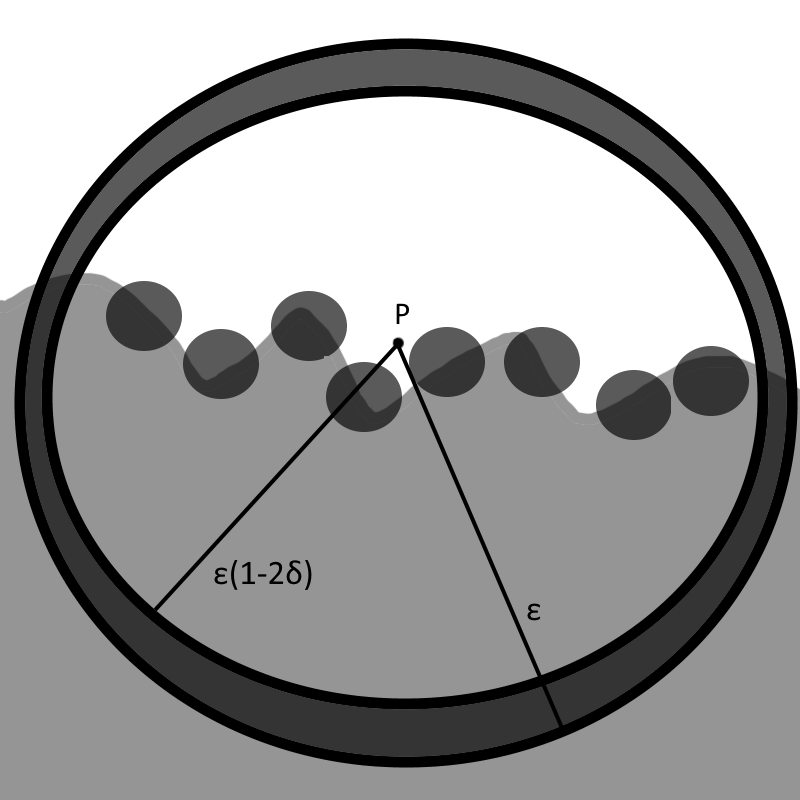
\includegraphics[width=0.4\textwidth]{covering lemma}
% \end{figure}

% \begin{sublemma}
% On $B_{1 - 2\sigma} \cap \{c\gamma^2 < \varphi < 1 - c\gamma^2\}$,
% $$(1_{V_0}(|\dif u| - Tu))_\varepsilon \lesssim_p \gamma |\dif u|_\varepsilon.$$
% \end{sublemma}
% \begin{proof}
% It follows from the definitions that for every $P \in B_\varepsilon$ and $Q \in V_0$, $\chi_\varepsilon(P - Q) \lesssim \varepsilon^{-d} \delta$,
% whence, by Proposition \ref{doubling dimension},
% \begin{align*}
% (1_{V_0}(|\dif u| - x\partial_zu))_\varepsilon &\lesssim \frac{\delta}{\varepsilon^d} \int_{B_\varepsilon} *|\dif u| \lesssim \frac{\delta}{\varepsilon}.
% \end{align*}
% Let $P \in B_\varepsilon$. Then by Lemma \ref{Giusti71}, there exists $c > 0$ such that if $\varphi \in (c\gamma^2, 1 - c\gamma^2)$, then there exists $Q \in \partial^* U$ such that $d(P, Q) < \varepsilon(1 - \gamma)$.
% If $d(Q, R) < \gamma\varepsilon/2$, then $d(P, R) < \varepsilon - \gamma\varepsilon/2$ and so $\chi_\varepsilon(P - R) \gtrsim \varepsilon^{-d}\gamma$ whenever $R \in B(Q, \gamma\varepsilon/2) =: W_0(P)$.
% We thus estimate
% $$\varepsilon^{-1} \gamma^{d - 1} \lesssim (1_{W_0(P)}|\dif u|)_\varepsilon \leq |\dif u|_\varepsilon$$
% and hence we obtain
% $$(1_{V_0}(|\dif u| - x\partial_zu))_\varepsilon(P) \lesssim \delta \gamma^{1 - d} |\dif u|_\varepsilon$$
% uniformly in $P$. Since $\delta = \gamma^d$, the claim holds.
% \end{proof}

%%%%%%%%%%%%%%%%%%%%%%%%%%%%%%%%%%%%%
\subsection{Mollification of sets of least perimeter}
Our goal for this section is to generalize \cite[Lemma 7.5]{Giusti77}, which reduces the study of sets of least perimeter to that of sets with $C^1$ perimeter.
We begin by recalling some known inequalities.

\begin{lemma}
Suppose that $u = 1_U$ where $U$ has locally finite perimeter, $w = u_\varepsilon$, and $V = \{w > y\}$ where $y \in (0, 1)$.
Then for any submanifold $\iota: E \to M$ and $0 < \varepsilon \lesssim 1$,
\begin{equation}\label{Giusti125}
x|E \cap (U \Delta V)| \leq \frac{1}{\min(y, 1 - y)} \int_E |w - u| \iota^*(\star 1).
\end{equation}
Moreover, if $0 < \tau \lesssim 1$, then
\begin{align}
\int_{B_\tau} \star |w - u| &\lesssim \varepsilon |B_{\tau + \varepsilon} \cap \partial^* U|, \label{Giusti711}\\
\int_{B_\tau} \star (|\dif w| - |\dif u|) &\lesssim |(B_{\tau + \varepsilon} \setminus B_\tau) \cap \partial^* U|. \label{Giusti712}
\end{align}
\end{lemma}
\begin{proof}
The estimate (\ref{Giusti125}) is a straightforward modification of \cite[Lemma 1.25]{Giusti77}.
The estimates (\ref{Giusti711}, \ref{Giusti712}) follow from \cite[Lemma 7.2]{Giusti77} where we use the fact that for $\tau \lesssim 1$, we can impose normal coordinates in which $\star 1$ is approximately the euclidean volume form.
\end{proof}

We now state the main mollification result.
On first reading it may help to fix $P_n = P$, $(x^\mu_n) = (x^\mu)$, $\omega = \star \dif x^\mu$, and $\Delta_n = 1$.

\begin{proposition}\label{mollifier quant}
Let $q < \min(1/8, 1/(4(d - 1)))$.
Let $(P_n)$ be a precompact sequence in $M$ and $0 < \Delta_n \lesssim 1$.
Let $U_n$ be a set of least perimeter in $B_n := B(P_n, \Delta_n)$, $(x^\mu_n)$ be a normal coordinate system at $P_n$, let $\psi^n$ be given by (\ref{d1 form}), and
$$\gamma_n := \Delta_n^{1 - d} \int_{B_n} \star |\psi^n| \cdot |\dif 1_{U_n}| - \dif 1_{U_n} \wedge \psi^n.$$
If $(\gamma_n) \in \ell^1$ then for almost every $t \in (0, 1)$ and every $n \in \NN$ there exists a set $V_n$ with $C^1$ boundary in $tB_n := B(P_n, t\Delta_n)$ such that for $n \gg 1$,
\begin{align}
|\partial V_n \cap tB_n| &\leq \eta(V_n, t\Delta_n) + o(\gamma_n \Delta_n^{d - 1}), \label{mollifier quant1}\\
||\partial^* U_n \cap tB_n| - |\partial V_n \cap tB_n|| &\ll \gamma_n \Delta_n^{d - 1}, \label{mollifier quant2}
\end{align}
on $B(P_n, t(1 - 2\sigma_n)\Delta_n)$, where $\sigma_n := \gamma_n^{1/(2(d - 1))}$, one has
\begin{equation}
\star(\normal_{V_n} \wedge \psi^n) \geq |\psi^n| \cdot (1 - o(\gamma^q)), \label{mollifier quant4}
\end{equation}
and for every $d-1$-form $\omega_n$ defined near $P_n$,
\begin{equation}\label{mollifier quant3}
\left|\int_{tB_n} \dif(1_{U_n} - 1_{V_n}) \wedge \omega_n\right| \ll \gamma_n \Delta_n^{d - 1} ||\omega_n||_{C^1}.
\end{equation}
\end{proposition}
\begin{proof}
In this proof, we shall assume that the constants furnished by the above results are uniform in $n$; this is possible by Remark \ref{independence of constants} and the compactness of $\overline{\{P_n: n \in \NN\}}$.

\proofpart{1}{Construction of $V_n$ and proof of (\ref{mollifier quant4})}
Draw $t$ uniformly at random, let $w_n := (u_n)_{\Delta_n \gamma_n^4}$, let $c, q$ be as in Proposition \ref{main mollifier lemma}, and let $a_n = c\gamma_n^2$, $b_n = 1 - c\gamma_n^2$.
By the coarea formula, Proposition \ref{Coarea2},
$$\int_{tB_n} \star |\dif w_n| = \int_0^1 |\partial^* \{w_n > y\} \cap tB_n| \dif y \geq \int_{a_n}^{b_n} |\partial^* \{w_n > y\} \cap tB_n| \dif y,$$
so by the mean value theorem, there exists $y_n \in (a_n, b_n)$ such that
$$|\partial^* \{w_n > y_n\} \cap tB_n| \leq \frac{1}{b_n - a_n} \int_{tB_n} \star |\dif w_n|.$$
We then set $V_n := \{w_n > y_n\}$, $v_n := 1_{V_n}$, so $V_n$ has $C^1$ boundary in $tB_n$ by (\ref{claim 2 on main mollifier lemma}), and by the above computation,
\begin{equation}\label{MVT mollifier}
|V_n \cap tB_n| \leq \frac{1}{1 - 2c\gamma_n^2} \int_{tB_n} \star |\dif w_n|.
\end{equation}
Since $\grad w_n$ is normal to the level sets of $w_n$, $\normal_{V_n} = \dif w_n/|\dif w_n|$.
Hence (\ref{mollifier quant4}) is a consequence of (\ref{claim on main mollifier lemma}).

\proofpart{2}{Auxiliary estimates}
Let $\Gamma_n := \partial(tB_n)$; we claim that almost surely,
\begin{align}
||u_n - v_n||_{L^1(\Gamma_n)} &\ll \Delta_n^{d - 1} \gamma_n \label{trace of vn} \\
|\partial V_n \cap tB_n| &\leq |\partial^* U_n \cap tB_n| + o(\Delta_n^{d - 1} \gamma_n). \label{difference of surface area}
\end{align}
To establish the claim, observe that by (\ref{Giusti711}) and Proposition \ref{doubling dimension},
$$\limsup_{n \to \infty} \Delta_n^{1 - d} \gamma_n^{-4} \int_{tB_n} \star |u_n - w_n| \lesssim \limsup_{n \to \infty} \Delta_n^{2-d} |\partial^* U_n \cap tB_n| \lesssim \sup_n \Delta_n \lesssim 1.$$
Differentiating in $t$, we see that
$$||u_n - w_n||_{L^1(\Gamma_n)} \ll \Delta_n^{d - 1} \gamma_n^3$$
almost surely. So by (\ref{Giusti125}),
$$||u_n - v_n||_{L^1(\Gamma_n)} \lesssim \gamma_n^{-2} ||u_n - w_n||_{L^1(\Gamma_n)} \ll \Delta_n^{d - 1} \gamma_n$$
almost surely, proving (\ref{trace of vn}).
Now let
$$f(s) = \sum_{n=1}^\infty \gamma_n \Delta_n^{1 - d} \int_{sB_n} \star |\dif u_n|.$$
Then $f' \geq 0$, and by Proposition \ref{doubling dimension}, $f(1) \lesssim \sum_n \gamma_n < \infty$.
So almost surely,
$$f(t + \gamma_n^4) - f(t) \lesssim \gamma_n^4$$
and hence
$$\int_{(t + \gamma_n^4)B_n \setminus tB_n} \star |\dif u_n| \lesssim \gamma_n^3 \Delta_n^{d - 1}.$$
From (\ref{Giusti712}) it follows that
$$\int_{tB_n} \star |\dif w_n| \leq \int_{tB_n} \star |\dif u_n| + o(\gamma_n^2).$$
By (\ref{MVT mollifier}) we conclude that (\ref{difference of surface area}) holds almost surely.

\proofpart{3}{Proof of (\ref{mollifier quant1}) and (\ref{mollifier quant2})}
The estimate (\ref{mollifier quant2}) is the conjunction of (\ref{trace of vn}), (\ref{difference of surface area}), and (\ref{a priori estimate 1});
(\ref{mollifier quant1}) is the conjunction of (\ref{mollifier quant2}), (\ref{a priori estimate 1}), the fact that $U_n$ has least perimeter, and (\ref{trace of vn}).

\proofpart{4}{Proof of (\ref{mollifier quant3})}
Integrating by parts,
$$\left|\int_{tB_n} \dif (u_n - v_n) \wedge \omega_n\right| \leq ||\omega_n||_{L^\infty} ||u_n - v_n||_{L^1(\Gamma_n)} + ||\dif \omega_n||_{L^\infty} \int_0^t ||u_n - v_n||_{L^1(\partial(sB_n))} \dif s.$$
By (\ref{trace of vn}),
$$\limsup_{n \to \infty} ||\omega_n||_{C^1}^{-1} \gamma_n^{-1} \Delta_n^{1 - d} \left|\int_{tB_n} \dif(u_n - v_n) \wedge \omega_n\right| \leq \limsup_{n \to \infty} \int_0^t \gamma_n^{-1} \Delta_n^{1 - d} ||u_n - v_n||_{L^1(\partial(sB_n))} \dif s.$$
Moreover, (\ref{trace of vn}) holds with $t$ replaced by almost any $s$, so
$$f_n(s) := \gamma_n^{-1} \Delta_n^{1 - d} ||u_n - v_n||_{L^1(\partial(sB_n))}$$
satisfies $(f_n) \in \ell^\infty([0, 1] \to L^\infty)$, and $f_n \to 0$ almost everywhere.
So by Fatou's lemma,
\begin{align*}
0 \leq \limsup_{n \to \infty} ||\omega_n||_{C^1}^{-1} \gamma_n^{-1} \Delta_n^{1 - d} \left|\int_{tB_n} \dif(u_n - v_n) \wedge \omega_n\right| &\leq \int_0^t \lim_{n \to \infty} f_n(s) \dif s = 0. \qedhere
\end{align*}
\end{proof}


%%%%%%%%%%%%%%%%%%%%%%%%%%%%%%%%%%%%%%%%%%%%%%
\section{Plateau's equation}\label{Plateau section}
Having shown that we can reduce the study of sets of least perimeter to sets with $C^1$ and approximately least perimeter, our next task is to represent such sets as graphs of approximate solutions to a Plateau-type equation.
For hyperbolic manifolds, Plateau's equation will be posed on $\Hyp^{d - 1}$, where we adopt the convention that $\Hyp^m = \RR^m$ for $m = 0, 1$.
To first order, Plateau's equation is nothing more than the Laplace-Beltrami equation on $\Hyp^{d - 1}$, so we can apply hyperbolic potential theory to prove the desired estimates.

\subsection{A flat connection}
Throughout the sequel we will need to ``average'' various tensor fields on $\Hyp^m$ for $m = d-1, d$.
In the euclidean case this can be accomplished by identifying every fiber $E_x$ of the tensor bundle with the fiber $E_0$ at $0$, and then viewing a tensor field $T$ as a vectorial function $\RR^d \to E_0$, and employ the vectorial integral $\int_{\RR^d} T \in E_0$.
Of course, the Riemann tensor is an obstruction to the existence of natural isomorphisms $E_x = E_0$ over $\Hyp^m$, so we must find isomorphisms $E_x \cong E_0$ which are ``approximately natural'' in some sense.

For $|x|$ small one can define the parallel propagator $E_x \to E_0$ in normal coordinates, and we believe that such a construction will give the same results that we will prove in the sequel.
However, since we will later have to restrict ourselves to the hyperbolic case anyways, we found it convenient to instead employ the elegant observation of Daskalopoulos--Uhlenbeck \cite{daskalopoulosPrep1} that one can embed $\Hyp^m$ in the Minkowski spacetime $\RR^{1, m}$ and employ the natural flat connection on $T\RR^{1, m}$ instead.

Recall that $\RR^{1,m}$ is $\RR^{1 + m}$ equipped with the Lorentz metric $\eta_{00} = -1$, $\eta_{ii} = 1$ for $i = 1, \dots, m$, and all other components $0$. TODO: Change the indices here
For the remainder of this paper we fix an identification of $\Hyp^m$ with the future branch of the unit timelike hyperboloid:
\begin{equation}\label{hyperboloid choice}
\Hyp^m \cong \{x \in \RR^{1,m}: \eta(x, x) = -1, x^0 > 1\}.
\end{equation}

Since the Riemann tensor of $\RR^{1,m}$ vanishes, the Levi-Civita connection on $T\RR^{1, m}$ is $\dif$, and once we have fixed (\ref{hyperboloid choice}), the restriction of the bundle $T\RR^{1, m}$ induces an isomorphism
$$T\RR^{1,m}|\Hyp^m = \Hyp^m \times \RR^{1,m},$$
a flat connection $\Dif$ on $\Hyp^m \times \RR^{1, m}$ defined by restricting $\dif$, and an exact sequence of quadratic bundles over $\Hyp^m$:
$$\begin{tikzcd}
0 \to (T\Hyp^m)^\perp \to \Hyp^m \times \RR^{1, m} \arrow[r,"\Pi"] & T\Hyp^m \to 0.
\end{tikzcd}$$
The next result follows from the definitions:

\begin{lemma}
The Christoffel symbols of $\Dif$ vanish with respect to any frame for $\Hyp^m \times \RR^{1,m}$ induced by a basis of $\RR^{1, m}$.
\end{lemma}

We henceforth adopt the convention that any $(\ell_1, \ell_2)$-tensor field on $\Hyp^m$ is to be identified with a map
$$\Hyp^m \to (\RR^{1, m})^{\otimes(\ell_1 + \ell_2)}$$
equipped with the connection $\Dif$.
In particular, it makes sense to define the vectorial integral
\begin{equation}\label{definition of vectorial integral}
\int_{\Hyp^m} T \otimes \vol \in (\RR^{1, m})^{\otimes (\ell_1 + \ell_2)}
\end{equation}
for every volume form $\vol$ and every tensor field $T \in L^1(\vol)$. More precisely, for every linear functional
$$\varphi: (\RR^{1, m})^{\otimes(\ell_1, \ell_2)} \to \RR,$$
we define 
$$\left(\varphi, \int_{\Hyp^m} T \otimes \vol\right) := \int_{\Hyp^m} (\varphi, T(x)) \vol(x)$$
where $(\varphi, T(x))$ makes sense since $T(x) \in (\RR^{1, m})^{\otimes (\ell_1 + \ell_2)}$.
Since $\Dif$ is flat, and the group $\SpOrth^+_{1, m}$ of properly orthochronous Lorentz transformations acts transitively on $\Hyp^m$, the integral (\ref{definition of vectorial integral}) is well-defined in the sense that any two different identifications (\ref{hyperboloid choice}) would merely transform the value of the integral by the action of $\SpOrth^+_{1, m}$.

\begin{definition}
The \dfn{average} in a ball $B \subset \Hyp^m$ is defined for tensor fields $T$ on $\Hyp^m$ by 
$$\avg_B T := \frac{1}{|B|} \int_B T \otimes (\star 1).$$
\end{definition}

The average is not a tensor field on $\Hyp^m$, but it can be transformed into one by applying the projection $\Pi$.
We write $\Pi_Q$ for the fiber of $\Pi$ over $Q \in \Hyp^m$, thus
\begin{equation}\label{projection formula}
\Pi_Q V = V + \eta(V, Q)Q.
\end{equation}

We now estimate $\Pi_Q: T_P\Hyp^m \to T_Q\Hyp^m$.
In the $m = 2$ case, which is essentially the same as the general case, these estimates already appear in \cite{daskalopoulosPrep1}, but at the time of writing that paper is still in preparation.

\begin{lemma}
Let $P, Q \in \Hyp^m$ and $t = \dist(P, Q)$. Then $P - Q$ is spacelike and 
$$\eta(P - Q, P - Q) = 2(\cosh t - 1) \in [t^2, t^2 \cosh t].$$
\end{lemma}
\begin{proof}
By acting $\SpOrth^+_{1, m}$ on $\RR^{1, m}$ we may assume that $P, Q$ are any two points connected by a geodesic of length $t$.
The geodesic $\gamma: [0, t] \to \Hyp^m$ such that
$$\gamma(s) = (\cosh s, \sinh s, 0, \dots, 0)$$
is spacelike and therefore satisfies
$$|\gamma| = \int_0^t \sqrt{\eta(\gamma'(s), \gamma'(s))} \dif s = \int_0^t \sqrt{\sinh^2 s - \cosh^2 s} \dif s = t.$$
Therefore we may assume that
\begin{align*}
P &= (1, 0, \dots, 0) \\
Q &= (\cosh t, \sinh t, 0, \dots, 0)
\end{align*}
and hence
\begin{align*}
\eta(P - Q, P - Q) &= \sinh^2 t - (\cosh t - 1)^2 = 2(\cosh t - 1). \qedhere 
\end{align*}
\end{proof}

\begin{lemma}
    Let $P, Q \in \Hyp^m$, $V \in T_P\Hyp^m$, and $W = \Pi_Q V$. Then
\begin{align*}
    |W| &\leq (1 + \eta(P - Q, P - Q)/2)|V|, \\
    |W - V| &\leq |V|\sqrt{\eta(P - Q, P - Q)} \sqrt{1 + \frac{1}{4} \eta(P - Q, P - Q)}.
\end{align*}
\end{lemma}
\begin{proof}
By (\ref{projection formula}),
$$|W|^2 = \eta(W, W) = \eta(V, V) + \eta(V, Q)^2$$
and $|W - V| = \eta(V, Q)$.
We therefore estimate 
\begin{align*}
\eta(V, Q)^2 &= \eta(V, \Pi_Q(P - Q))^2 = \eta(V, P - Q + \eta(P - Q, Q)Q).
\end{align*}
Since every tangent vector to $Q$ is spacelike,
$$\eta(V, P - Q + \eta(P - Q, Q)Q) \leq \eta(W, W)(\eta(P - Q, P - Q) + \eta(Q - P, Q)^2)$$
and as 
$$\eta(Q - P, Q) = \frac{1}{2}\eta(P - Q, P - Q),$$
we conclude 
\begin{align*}
\eta(V, Q)^2 &\leq \eta(V, V) \eta(P - Q, P - Q) \left[1 + \frac{1}{4} \eta(P - Q, P - Q)\right]. \qedhere
\end{align*}
\end{proof}

TODO: Get a formula for $\Dif$ versus $\dif$.

Since we are going to be interested in averages, we will need to study various Laplacian operators acting on tensor fields on $M$.
The lack of a canonical choice of Laplacian is measured by the \emph{non}commutativity of the diagram 
$$\begin{tikzcd}
C^\infty(M, T'M)_{\mathrm{cl}} \arrow[hookrightarrow]{r} \arrow["\dif^*"]{d} &
C^\infty(M, \RR^{1, m}) \arrow["\Dif"]{r} &
C^\infty(M, \RR^{1, m} \otimes T'M) \arrow["\Dif^*"]{d} \\
C^\infty(M, \RR) \arrow["\dif"]{r} &
C^\infty(M, T'M) \arrow[hookrightarrow]{r} &
C^\infty(M, \RR^{1, m})
\end{tikzcd}$$
where $C^\infty(M, T'M)_{\mathrm{cl}}$ is the space of closed $1$-forms on $M$, $\dif^*$ is the coderivative (so $\dif \circ \dif^*$ is the Hodge-Laplace operator on closed forms), and $\Dif^*$ is the adjoint
$$\Dif^* (F \otimes \alpha) = \tr_g (\Dif F \otimes \alpha)$$
(so $\Dif^* \circ \Dif$ is the Laplacian with respect to the flat connection $\Dif$).
TODO: Who cares?

\begin{definition}
A $\flat$-\dfn{harmonic form} is a differential form $\alpha$ on $M$ such that
$$\dif \alpha = \Dif^* (\Dif \alpha) = 0.$$
\end{definition}

\begin{lemma}
Let $u$ be a harmonic function on $M$. Then $\Dif^* \Dif \dif u = ...$
\end{lemma}

\begin{lemma}[$\flat$-mean value property]
Let $\alpha$ be a $\flat$-harmonic form. Then for $P \in M$ and $r > 0$<
$$\alpha(P) - \avg_{B(P, r)} \alpha = TODO.$$
\end{lemma}
\begin{proof}

\end{proof}

\subsection{Plateau energy}
% choose coords...

% \begin{lemma}
% Let $M$ be a hyperbolic manifold and $(P, V) \in TM$.
% Then there exist coordinates $(x^\mu)$ on $M$ such that $x(P) = 0$, $\partial_0(P) = V$, and
% and the metric takes the form $\partial_0 g_{\mu\nu} = 0$, $g_{0i} = g_{i0} = 0$, $\partial_k g_{ij}(0) = 0$, and $g_{\mu\nu}(0) = \delta_{\mu\nu}$.
% \end{lemma}
% \begin{proof}
% Using the upper half-space model, there exist coordinates $(\underline x^\mu)$ on $M$ so that
% $$\underline g_{\mu\nu} = (\underline x^1)^{-2} \delta_{\mu\nu},$$
% $\underline x^0(P) = 0$, $\underline x^1(P) = 1$, and $\underline \partial_0(P) = V$.
% To construct a coordinate system which is more adapted to the Plateau equation we define $x^0 = \underline x^0$.
% Using the flow of $\partial_0$, we obtain maps
% $$\phi_c: \{x^0 = 0\} \to \{x^0 = c\}.$$
% Moreover on $\{x^0 = 0\}$ the metric takes the form $\underline g_{ij} = (\underline x^1)^{-2} \delta_{ij}$, thus $\{x^0 = 0\}$ embeds isometrically in $\Hyp^{d - 1}$.
% We therefore choose $P$-based normal coordinates $(x^i)$ for $\Hyp^{d - 1}$ and extend them to a neighborhood of $\{x^0 = 0\}$ by pulling them back using $\phi_c$.
% We recall that $\partial_0 = \underline \partial_0$ is a Killing field.

% Since $(\partial_0)^\flat_\mu = g_{\mu 0}$, one has the Killing equation
% $$\partial_\mu g_{\nu 0} + \partial_\nu g_{\mu 0} - 2\Gamma_{\mu \nu}^\lambda g_{\lambda 0} = 0.$$
% However,
% $$2 \Gamma^\lambda_{\mu \nu} g_{\lambda 0} = \partial_\nu g_{0 \mu} + \partial_\mu g_{0 \nu} - \partial_0 g_{\mu \nu}$$
% and so we conclude $\partial_0 g_{\mu \nu} = 0$.
% Moreover, $x^0 = \underline x^0$ and $\underline \partial_0$ is orthogonal to $\{\underline x^0 = c\}$ which implies that, since $\partial_i$ is tangent to $\{\underline x^0 = c\}$, $g_{0i} = g_{i0} = 0$.
% The remaining two conditions are characteristic of normal coordinates on $\Hyp^{d - 1}$.
% \end{proof}

% In other words, the metric $g$ in the above lemma takes the form
% $$g = \begin{bmatrix}
% 1 + O(r) & 0\\
% 0 & I + O(r^2)
% \end{bmatrix}$$
% where $I$ is the identity matrix. At $P$, the only nonzero components of $(\partial_\lambda g_{\mu\nu})$ are of the form $\partial_i g_{00}$ and so the only nonzero Christoffel symbols there are $\Gamma^0_{0i} = \Gamma^0_{i0} = g^{00} \partial_i g_{00}/2$ and $\Gamma_{00}^i = -\partial^i g_{00}$.

Our next task is to construct Plateau's equation as the Euler-Lagrange equation of a certain Lagrangian on $\Hyp^{d - 1}$.
To accomplish this we first identify a coordinate condition which makes Plateau's equation take a particularly simple form.

\begin{definition}
Let $M = (M, g)$ be a hyperbolic manifold equipped with a coordinate system $(x^\mu)$.
We say that $g$ is in \dfn{Killing gauge} if it takes the form 
$$g = g_{00} \dif x^0 \otimes \dif x^0 + g_{ij} \dif x^i \otimes \dif x^j$$
for $i, j = 1, \dots, d - 1$, and $\partial_0$ is an infinitesimal generator of translations.
\end{definition}

\begin{lemma}
If $g$ is in Killing gauge, then $\partial_0 g_{\mu\nu} = 0$ and $(\{x^0 = c\}, (g_{ij}))$ is locally isometric to $\Hyp^{d - 1}$.
\end{lemma}
\begin{proof}
The equation $\partial_0 g_{\mu\nu} = 0$ is equivalent to $\partial_0$ being a Killing field. This follows from the fact that $(\partial_0)^\flat_\mu = g_{\mu 0}$ and the Killing equation 
$$\partial_\mu g_{\nu 0} + \partial_\nu g_{\mu 0} - 2\Gamma_{\mu \nu}^\lambda g_{\lambda 0} = 0,$$
where we can expand the Christoffel symbols as
$$2 \Gamma^\lambda_{\mu \nu} g_{\lambda 0} = \partial_\nu g_{0 \mu} + \partial_\mu g_{0 \nu} - \partial_0 g_{\mu \nu}.$$
Moreover, since $\partial_0$ is an infinitesimal generator of translations, we can identify $x^0$ with the vector field $\tilde x^0$ in the half-space model $\tilde g_{\mu\nu} = (\tilde x^1)^{-2} \delta_{\mu\nu}$, thus $(\{x^0 = c\}, (g_{ij}))$ is locally isometric to $(\{\tilde x^0 = 0\}, (\tilde g_{ij}))$ and $\tilde g_{ij} = (\tilde x^1)^{-2} \delta_{ij}$ so $(\{\tilde x^0 = 0\}, (\tilde g_{ij})) \cong \Hyp^{d - 1}$.
\end{proof}

\begin{lemma}[existence of Killing gauge]\label{existence of Killing gauge}
Let $M$ be a hyperbolic manifold, $(P, V) \in TM$, and $(y^i)$ are coordinates on an open subset $\Omega$ of $\Hyp^{d - 1}$ based at some point $Q$.
Then, possibly after shrinking $\Omega$, we can find an embedding $\iota: \Omega \to \Hyp^d$ and coordinates $(x^\mu)$ on $\Hyp^d$ based at $P$ such that:
\begin{enumerate}
\item $\iota(Q) = P$ and $\iota^* (x^i) = y^i$ for $i = 1, \dots, d - 1$,
\item $(g_{\mu\nu})$ is in Killing gauge,
\item $\iota_* (\Omega) = \{x^0 = 0\}$, and 
\item $\partial_0(P) = V$.
\end{enumerate}
\end{lemma}
\begin{proof}
Since $M$ is hyperbolic and the statement is local, we may assume that $M = \Hyp^d$ in the half-space model $\tilde g_{\mu\nu} = (\tilde x^{d - 1})^{-2} \delta_{\mu\nu}$, $P = (0, \dots, 0, 1)$, and $V = \tilde \partial_0(P)$.
We then set $x^0 = \tilde x^0$.
In particular, $\partial_0$ is a Killing field and is orthogonal to $\{x^0 = c\}$ for every $c$.
In the coordinates $(\tilde x^\mu)$, the induced metric on $\{x^0 = 0\}$ is $\tilde g_{ij} = (\tilde x^{d - 1})^{-2} \delta_{ij}$, which is hyperbolic, so $\{x^0 = 0\}$ is locally isometric to $\Hyp^{d - 1}$.
The coordinate fields $\partial_i$ are tangent to $\Hyp^{d - 1}$ and therefore orthogonal to $\partial_0$.
Therefore the desired embedding $\iota$ exists and maps $\Omega$ onto a small neighborhood of $P$ in $\{x^0 = 0\}$.
\end{proof}

Suppose that $(x^\mu)$ is in Killing gauge, $\Omega \subseteq \Hyp^{d - 1}$ is open, and we have an identification
$$\Omega \cong \{x^0 = 0\};$$
we will not explicitly write pullbacks or pushforwards for this identification.
Suppose further that
$$\omega: \Omega \to \RR$$
is a $C^1$ function. Then one has a graph
$$N = \{(\omega(x), x) \in M: x \in \Omega\}.$$
Let $\Psi: \Omega \to N$ be the diffeomorphism $\Psi(x) = (\omega(x), x)$. Then
$$\dif \Psi = \begin{bmatrix}
\dif \omega \\
I
\end{bmatrix}$$
so
\begin{align*}
(\Psi^* g)_{ij} &= g(\dif \Psi \cdot \partial_i, \dif \Psi \cdot \partial_j) = g_{\mu\nu} \dif \Psi^\mu_i \dif \Psi^\nu_j \\
&= g_{\mu\nu} (\delta^\mu_0 \partial_i \omega + \delta^\mu_i)(\delta^\nu_0 \partial_j \omega + \delta^\mu_j)\\
&= \Psi^* (g_{ij}) + \Psi^* (g_{00}) \partial_i \omega \partial_j \omega.
\end{align*}
Here $(\Psi^* g)_{ij}$ are components of the pullback metric but $\Psi^* (g_{\mu\nu})$ are pullbacks of the components of the metric.
Using the Killing nature of $\partial_0$ we can eliminate the pullbacks on the components, thus
$$\Psi^* g = g_{ij} \dif x^i \otimes \dif x^j + g_{00} \dif \omega \otimes \dif \omega.$$
The only independent component of the volume form of the pullback metric $\Psi^* g$ is
$$\sqrt{\det \Psi^* g} = \sqrt{\det ((g_{ij}))} \sqrt{1 + g_{00} |\dif \omega|_{g^{-1}}^2}$$
by the Weinstein-Aronsazjn theorem.

\begin{definition}
Suppose that $(M, g)$ is a hyperbolic manifold and $g$ is in Killing gauge.
Let $\Omega \subseteq \Hyp^{d - 1}$ and let $\omega: \Omega \to \RR$ be $C^1$. Then the \dfn{Plateau energy} of $\omega$ is the $d-1$-form
$$\Lagrange[\dif \omega] = \star \sqrt{1 + F |\dif \omega|^2},$$
on $\Hyp^{d - 1}$ and $F$ is the pullback of $g_{00}$ on $\{x^0 = 0\} \subset M$ to $\Hyp^{d - 1}$.

The \dfn{Plateau equation} is the Euler-Lagrange equation for the Plateau energy, and a variational solution of the Plateau equation is called a \dfn{minimal graph}.
\end{definition}

It follows from the definitions that, if $N$ is the graph of $\omega$, then $\Lagrange[\dif \omega]$ is the pullback of the volume form on $N$ by $\Psi$.
In particular, minimal graphs have no mean curvature.

\begin{lemma}
The Plateau equation is the elliptic PDE on $\Hyp^{d - 1}$,
\begin{equation}\label{Plateau eqn}
\Delta \omega + \frac{\sqrt{1 + F |\nabla \omega|^2}}{F} g\left(\nabla \frac{F}{\sqrt{1 + F |\nabla \omega|^2}}, \nabla \omega\right) = 0.
\end{equation}
\end{lemma}
\begin{proof}
Consider a variation $\omega$ with $\phi = -\dot \omega$ compactly supported in $\Hyp^{d - 1}$:
\begin{align*}
\frac{\dif}{\dif t} \Lagrange[\dif \omega] &= \int_{\Hyp^{d - 1}} \star \partial_t \sqrt{1 + F |\nabla \omega|^2} \\
&= -\int_{\Hyp^{d - 1}} \star \frac{F g(\nabla \phi, \nabla \omega)}{\sqrt{1 + F|\nabla \omega|^2}} \\
&= \int_{\Hyp^{d - 1}} \star \phi\left[\frac{F}{\sqrt{1 + F |\nabla \omega|^2}} \Delta \omega + g\left(\nabla \frac{F}{\sqrt{1 + F |\nabla \omega|^2}}, \nabla \omega\right)\right]. \qedhere
\end{align*}
\end{proof}

\begin{lemma}\label{C1 implies smooth}
Let $U$ be a set of least perimeter in a hyperbolic manifold, and assume that $\normal_U$ extends to a continuous $1$-form on $\partial U$.
Then $\partial U$ is $C^\infty$.
\end{lemma}
\begin{proof}
By Proposition \ref{locality of Caccioppoli}, $\partial U$ is $C^1$ and has no mean curvature.
Let $P \in \partial U$, and use Lemma \ref{existence of Killing gauge} to choose coordinates based at $(P, \normal_U(P))$ for which $g$ is in Killing gauge.
In these coordinates, $\partial U$ is a minimal graph and by elliptic regularity is $C^\infty$.
\end{proof}

%%%%%%%%%%%%%%%%%%%%%%%%%%%%%%%%%
\subsection{Hyperbolic harmonics}
Linearizing (\ref{Plateau eqn}) about $||\omega||_{C^1} \ll 1$, we arrive at the Laplace-Beltrami equation $\Delta \omega = 0$ on $\Hyp^{d - 1}$, $d \geq 2$.
We therefore will study of harmonic functions on $\Hyp^{d - 1}$.
The results of this section are trivial for $d = 2$ and so the reader who is only interested in application to surfaces can skip this section entirely.
Henceforth, we assume $d \geq 3$.

In polar coordinates, we have 
$$\sinh^2 r \Delta = \sinh^2 r \frac{\partial^2}{\partial r^2} + (d - 2) \sinh r \cosh r \frac{\partial}{\partial r} - L$$
where $-L$ is the Laplace-Beltrami operator on $\Sph^{d - 2}$.
From the separation ansatz $u(r, \theta) = v(r) Y(\theta)$ we have if $u$ is harmonic that 
$$0 = \sinh^2 r \Delta u(r, \theta) = Y(\theta) (\sinh^2 r v''(r) + (d - 2) \sinh r \cosh r v'(r)) - v(r) LY(\theta)$$
which decouples into the system 
\begin{align}
\sinh^2 r v''(r) + (d - 2) \sinh r \cosh r v'(r) - \lambda vR(r) &= 0 \label{radial hyperbolic harmonic} \\
LY(\theta) - \lambda Y(\theta) &= 0
\end{align}
where $\lambda$ ranges over $\Spec L$, thus $\lambda = \lambda_\ell := \ell(\ell + d - 3)$ for some quantum number $\ell \in \NN$ and after rescaling $Y$ by some constant $\alpha > 0$ (and thus rescaling $v$ by $1/\alpha$), $Y$ is a spherical harmonic $Y = Y^k_\ell$ for some quantum number $k \in \NN$.

\begin{definition}
By a \dfn{hyperbolic harmonic} we mean a function of the form 
$$u(r, \Theta) = v(r) Y^k_\ell(\theta)$$
where $v$ is a \dfn{radial hyperbolic harmonic} of quantum number $\ell$, i.e. a solution of (\ref{radial hyperbolic harmonic}) with $\lambda = \lambda_\ell$.
\end{definition}

\begin{lemma}
For every $\ell \in \NN$ we can find hyperbolic harmonics $v_\ell^m$, $m \in \{0, 1\}$, of quantum number $\ell$, so that $(v_\ell^m Y^k_\ell)_{\ell, m, k}$ is an orthonormal basis of the space of harmonic functions on any ball centered on the origin.
\end{lemma}
\begin{proof}
By standard elliptic theory the hyperbolic harmonics are dense.
For fixed $\ell$ the space of smooth solutions to (\ref{radial hyperbolic harmonic}) is $\leq 2$-dimensional and so $v_\ell^m$ are given by the Gram-Schmidt algorithm.
Now if we set $u_\ell^{m, k}$ we have for a ball $B_r$, 
$$\int_{B_r} \star u_{\ell_1}^{m_1, k_1} u_{\ell_2}^{m_2, k_2} = \langle v_{\ell_1}^{m_1}, v_{\ell_2}^{m_2}\rangle \int_{\Sph^{d - 1}} Y_{\ell_1}^{k_1} Y_{\ell_2}^{k_2} \dif \sigma.$$
The spherical integral vanishes unless $(\ell_1, k_1) = (\ell_2, k_2)$.
If $\ell_1 = \ell_2$ then the inner product vanishes unless $m_1 = m_2$.
\end{proof}

\begin{lemma}
If $u$ has a double zero at $P \in \Hyp^{d - 1}$ and $\Delta u = 0$, then 
$$\int_{B(P, r/2)} \star |\dif u|^2 \leq \frac{1}{2^{d + 1}} \int_{B(P, r)} \star |\dif u|^2.$$
\end{lemma}
\begin{proof}

\end{proof}



% \subsection{Laplacian approximation}
% For this subsection only, let $g$ be a Riemannian metric on $\RR^{d - 1}$ which is normal based at $0$.
% Thus if $d = 2$, $g_{\mu\nu} = \delta_{\mu\nu}$ and all the results of this section are vacuously true, so for the remainder of this section only we assume $d \geq 3$.
% In particular, the reader who is only interested in our application to closed hyperbolic surfaces can skip this section entirely.

% We will compare the behavior of the Laplace-Beltrami equation
% $$\Delta u = \nabla^\mu \partial_\mu u = 0$$
% of $g$ to the euclidean Laplace equation $Lu = 0$, in the limiting case $r + ||u||_{C^1} \ll 1$ where $r$ is the radial coordinate.

% \begin{definition}
% The \dfn{Laplacian approximation} of a $g$-harmonic function $u$ on $B_r$ is the euclidean-harmonic function $v$ such that $u = v$ on $\partial B_r$.
% \end{definition}

% \begin{lemma}
% Let $u$ be a $g$-harmonic function. Then the Laplacian approximation $v$ on $B_r$ satisfies 
% $$||u - v||_{L^\infty} \lesssim r^3 ||u||_{\dot W^{1, \infty}} + r^4 ||u||_{\dot W^{2, \infty}}.$$
% \end{lemma}
% \begin{proof}
% Expanding $\Delta$ near $0$ we have 
% $$\Delta = (\delta^{\mu\nu} + O(r^2)^{\mu\nu})(\partial_\mu \partial_\nu - \Gamma_{\mu\nu}^\lambda \partial_\lambda).$$
% Since all Christoffel symbols vanish at $0$, we obtain from Taylor's formula and the fact that $L = \delta^{\mu\nu} \partial_\mu \partial_\nu$ that
% $$\Delta - L = O(r|\partial| + r^2|\partial|^2).$$
% If we set $w = u - v$, then $w$ solves the equation 
% $$Lw = O(r|\partial| + r^2|\partial|^2)u$$
% and has homogeneous Dirichlet data. So if $G: B_r \times B_r \to \RR$ is the Green function of $L$,
% $$w(x) = \int_{B_r} G(x, y) O(|y|\cdot ||u||_{\dot W^{1, \infty}} + |y|^2 \cdot ||u||_{\dot W^{2, \infty}}) \dif y$$
% and hence by H\"older's inequality,
% \begin{equation}\label{Linfty LBL error bound}
% ||w||_{L^\infty} \lesssim ||G||_{L^\infty;L^1} (r||u||_{\dot W^{1, \infty}} + r^2 ||u||_{\dot W^{2, \infty}}).
% \end{equation}
% The maximizer of $||G(x, \cdot)||_{L^1}$ is $x = 0$, and $L$ admits a fundamental solution since $d \geq 3$, whose radial profile we denote by $\Phi$. Therefore
% $$||G||_{L^\infty;L^1} = ||G(0, \cdot)||_{L^1} = \int_{B_r} \Phi(|y|) - \Phi(r) \dif y.$$
% If $d = 3$, then
% $$\int_{B_r} \Phi(|y|) - \Phi(r) \dif y \lesssim \int_0^r s(\log r - \log s) \dif s \lesssim r^2,$$
% while for $d \geq 4$,
% $$\int_{B_r} \Phi(|y|) - \Phi(r) \dif y \lesssim \int_0^r s^{d - 2}(s^{3 - d} - r^{3 - d}) \dif s \lesssim r^2 \left[\frac{1}{3} - \frac{1}{d}\right] \lesssim r^2.$$
% Plugging this into (\ref{Linfty LBL error bound}) gives the desired result.
% \end{proof}






\begin{proposition}\label{dGL Laplace}
de giorgi lemma for harmonics
\end{proposition}




%%%%%%%%%%%%%%%%%%%%%%%%%%%%%%%%%%%%%%

% \section{Regularity of minimal hypersurfaces}\label{de Giorgi section}
% In this section we shall prove Theorem \ref{main lma}.
% The key step, as in \cite{Miranda66}, is to prove a de Giorgi lemma for sets of least perimeter by exploiting the gains of Proposition \ref{dGL Laplace}, which we now formulate.

% \begin{definition}
% The \dfn{excess} of a set $U$ of locally finite perimeter in a ball $B$, with indicator function $u = 1_U$, is
% $$\Exc_B U := r^{1 - d}\left[\int_B \star |\dif u| - \left|\int_B \dif u \otimes (\star 1)\right|\right].$$
% \end{definition}

% \begin{proposition}[de Giorgi's lemma]\label{dGL final}
% Suppose that $M$ is locally homogeneous, $d \leq 7$, $K \subseteq M$ is compact, and $U$ is a set of least perimeter. Then for every $P \in K$,
% $$\Exc_{B(P, r)} U \lesssim_{U, K} r.$$
% \end{proposition}

% The excess measures how badly the conormal $1$-form $\normal = \normal_U$ fails to be ``constant'' and so functions as a sort of averaged version of the second fundamental form of $\partial U$.
% As there are multiple, nonequivalent notions of excess in the literature, we stress that this notion of excess is a generalization of the notion defined by de Giorgi when he first proved his lemma \cite{deGiorgi61}; it is not equivalent to the notion used by Allard \cite{Allard72} in the proof of his regularity theorem, c.f. \cite{colding2011course}.

% The proof of Proposition \ref{dGL final} generalizes the proof of \cite[Teorema 5.7]{Miranda66}; it appears in \S\ref{dGL proof}.
% In \S\ref{main lma proof} we apply de Giorgi's lemma and a standard induction-on-scale argument, following \cite[Teorema 6.5]{Miranda66}, to conclude Theorem \ref{main lma}.

% \subsection{The excess}
% We first study the properties of the excess.

% \begin{definition}
% Let $U$ be a set of locally finite perimeter and $u = 1_U$.
% The \dfn{approximate conormal} $1$-form $\widetilde \normal_r$ to $U$ at scale $r$ is defined for $P \in \partial U$ by choosing a maximizer $\xi \in \SpOrth(T_PM)$ of $\int_{B(P, r)} \dif u \wedge \psi_\xi/|\psi_\xi|$ and setting
% $$\widetilde \normal_r(P) = \frac{1}{|\partial^* U \cap B(P, r)|} \left[\int_{B(P, r)} \dif u \wedge \frac{\psi_\xi}{|\psi_\xi|}\right] \dif x^0_\xi \in T'_PM.$$
% \end{definition}

% By compactness of $\SpOrth(T_PM)$ there exists $\xi \in \SpOrth(T_PM)$ which maximizes $\int_{B(P, r)} \dif u \wedge \psi_\xi/|\psi_\xi|$.
% Moreover this maximizer is unique if $P \in \overline{\partial^* U}$, so the approximate conormal $1$-form is well-defined as a measurable section of $T'M$ along $\partial U$ by Proposition \ref{locality of Caccioppoli}.
% Since it is defined by an averaging procedure, $\widetilde \normal_r$ is also continuous.
% By (\ref{Lebesgue point definition}), $\widetilde \normal_r \to \normal_U$, $\star|\dif u|$-almost everywhere.
% Moreover, since $(x^\mu_\xi)$ is normal based at $P$, and $\widetilde \normal_r(P) \in T'_PM$,
% $$|\widetilde \normal_r(P)| \int_{B(P, r)} \star |\dif u| = \left|\int_{B(P, r)} \dif u \otimes (\star 1)\right|.$$
% In particular,
% \begin{equation}\label{excess vs 1form}
% \Exc_{B(P, r)} U = r^{1 - d} (1 - |\widetilde \normal_r(P)|) \int_{B(P, r)} \star |\dif u|.
% \end{equation}

% \begin{lemma}[de Giorgi's lemma, $C^1$ case]
% beep
% \end{lemma}

% \subsection{de Giorgi's lemma}\label{dGL proof}
% We now complete the proof of Proposition \ref{dGL final} using a compactness-and-contradiction argument.
% Suppose that de Giorgi's lemma is false for some sets $U$ of least perimeter and $K$ compact. Then we can choose $P_n \in K$ and $r_n > 0$ so that $r_n \to 0$, but
% $$\gamma_n := \Exc_{B(P_n, r_n)} U$$
% satisfies
% \begin{equation}\label{contradict dGL}
% \gamma_n \geq nr.
% \end{equation}
% In what follows we shall pass to subsequences repeatedly as necessary.

% \begin{claim}
% We may assume $(\gamma_n) \in \ell^1$.
% \end{claim}
% \begin{proof}
% If not, then there exists $\delta > 0$ such that $\gamma_n \geq \delta$.
% Let $N = \overline{\partial^* U} \cap K$.
% If $(P_n)$ converges to a point in the open set $M \setminus N$, then since $N$ is the support of $\star |\dif u|$, $\gamma_n$ is eventually $0$.
% Therefore the assumption $\gamma_n \geq \delta$ implies that every convergent subsequence of $(P_n)$ converges to a point in $N$.
% In particular we may assume that $(P_n)$ converges to some $P \in N$. By definition of $N$ there exist $Q_n \in \partial^* U \cap K$ converging to $P$, and by Proposition \ref{blowup theorem}, there exist (possibly nonunique) blowups $v_n: T_{Q_n}M \to \RR$ of $u$.

% We choose normal coordinates based at $Q_{n^*}$ for some $n^* \geq 1$, and let $\widetilde \normal_r$ be the induced approximate conormal.
% Then $\widetilde \normal_r$ is continuous
% \end{proof}


% \subsection{Proof of main theorem}\label{main lma proof}
% Let $U$ be a set of least perimeter, and $P \in \partial U$.
% We shall show that in the limit $r \to 0$, $(\widetilde \normal_r)$ is a locally uniformly Cauchy net.
% If this is true, then $\normal$ is a continuous section of $T'M$ on $\partial U$, so by Lemma \ref{C1 implies smooth}, $\partial U$ is smooth.

% To show the Cauchy condition, we TODO: Approximate $\widetilde \normal_r$ by normal coordinates that agree with $\Exc_r$ (eats a loss of $r^2$) and then use Giusti82


\printbibliography

\end{document}
